\documentclass[12pt,a4paper]{article}
\usepackage[utf8]{inputenc}
\usepackage[german]{babel}
\usepackage[T1]{fontenc}
\usepackage{amsmath}
\usepackage{amsfonts}
\usepackage{amssymb}
\usepackage{graphicx}
\usepackage[left=2.5cm,right=2.5cm,top=2cm,bottom=2cm]{geometry}
\author{Gruppe C14 \\ Julián Häck, Martin Koytek, Lars Wenning, Erik Zimmermann}
\usepackage{float}
\usepackage{subfigure}
\begin{document}
\section{Widerstand, Teilversuch 4.1}
\subsection{Versuchsbeschreibung}
Aus dem Ohm'schen Gesetz folgt:
\[R=\frac{U}{I}\]
Aus der am Widerstand anliegenden Spannung $U$ und dem durch den Widerstand fließenden Strom $I$ wird hier der Wert für den Widerstand $R$ berechnet.
\subsection{Versuchsaufbau und Durchführung}
%Genaue Beschreibung der verwendeten Aufbauten unter Verwendung von Skizzen oder Photos
%Beschreibung der Messwerterfassungseinstellungen (eingestellte %Messzeiten, Messbedingungen,
%Trigger, Anzahl der Messungen) und der Durchführung der Versuche. (max. 1 Seite)
\begin{center}
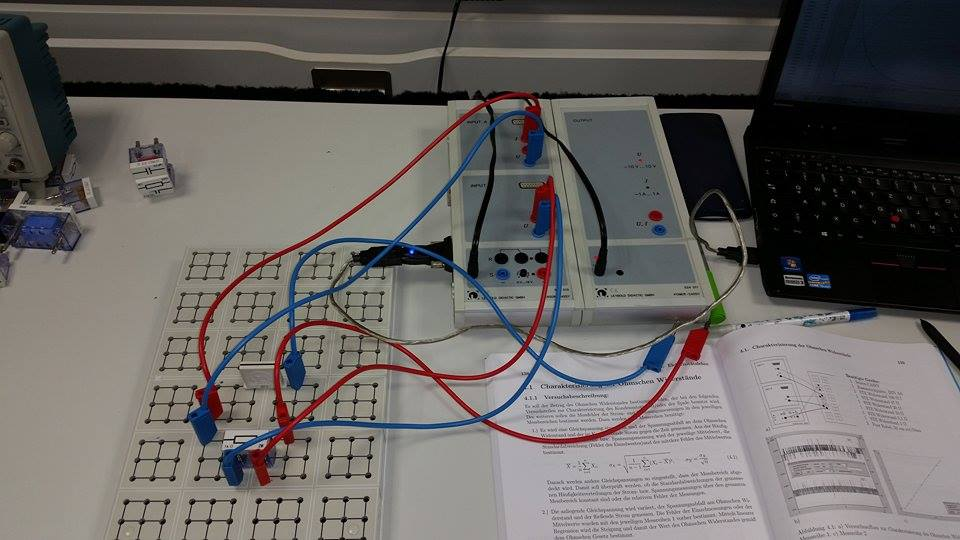
\includegraphics[scale=0.35]{12000155_1207085929316467_1534534399_n.jpg}
\end{center}

Der erste Versuch bestand aus Rauschmessungen, in denen jeweils die Spannung $U$ und der Strom $I$ bei konstanten Eingangsspannungen aufgezeichnet wurde.
Bei den Messungen wurden jeweils 1000 Werte über einen Messzeitraum von $10ms$ aufgezeichnet. Die Spannung wurde in einem Messbereich von $-10V$ bis $+10V$ und der Strom von $-0,1A$ bis $+0,1A$ gemessen.
Anschließend wurde die Spannung variiert, um den Messbereich abzudecken und eine eventuelle relative Abhängigkeit des Fehlers von der Spannung auszuschließen. 

\subsection{Versuchsauswertung}
Aus den Daten der Strom- und Spannungsmessung wurden anschließend die Mittelwerte von $U$ und $I$ mit deren statistischen Fehler bestimmt.
Die statistischen Fehler wurden dann mittels Fehlerfortpflanzung der aus den Herstellerangaben entnommenen $\sigma_{U,sys}$ und $\sigma_{I,sys}$ errechnet. 
Aus den jeweils berechneten Werten für $R$ konnte dann der Mittelwert und damit das Endergebnis angegeben werden.
\subsubsection{Rohdaten}
\begin{figure}
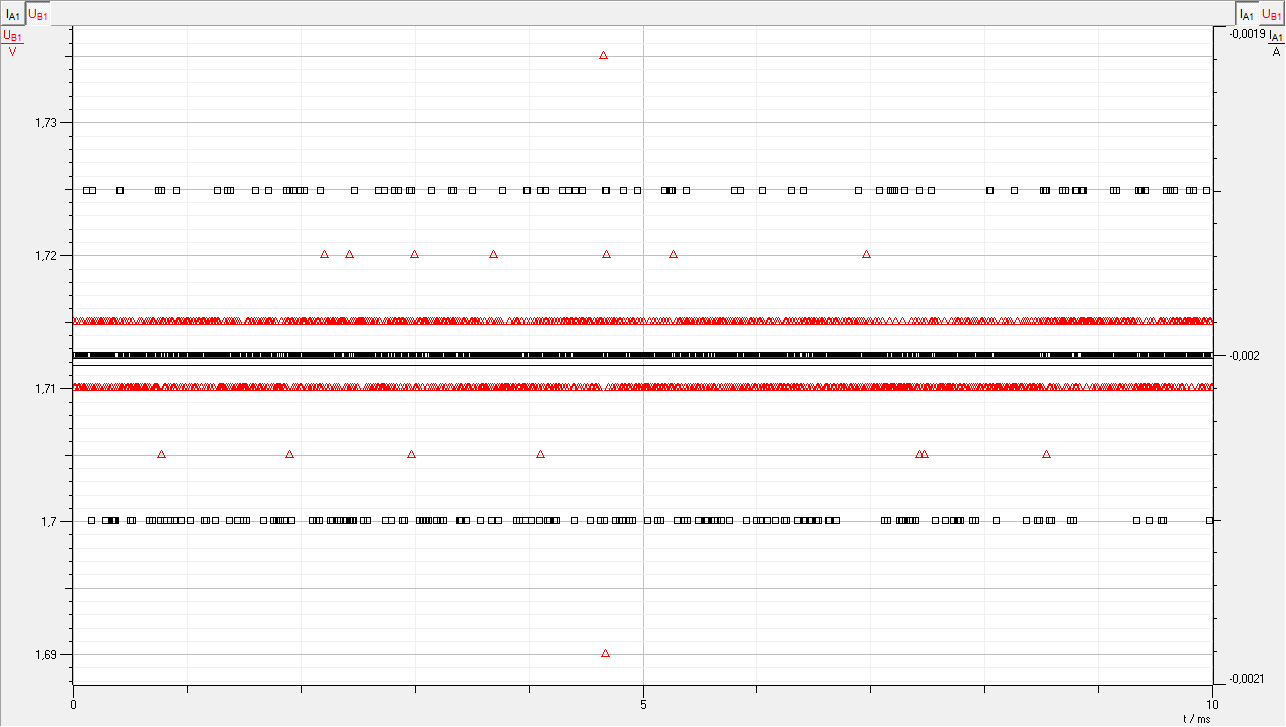
\includegraphics[scale=0.6]{Rauschmessung1.png}
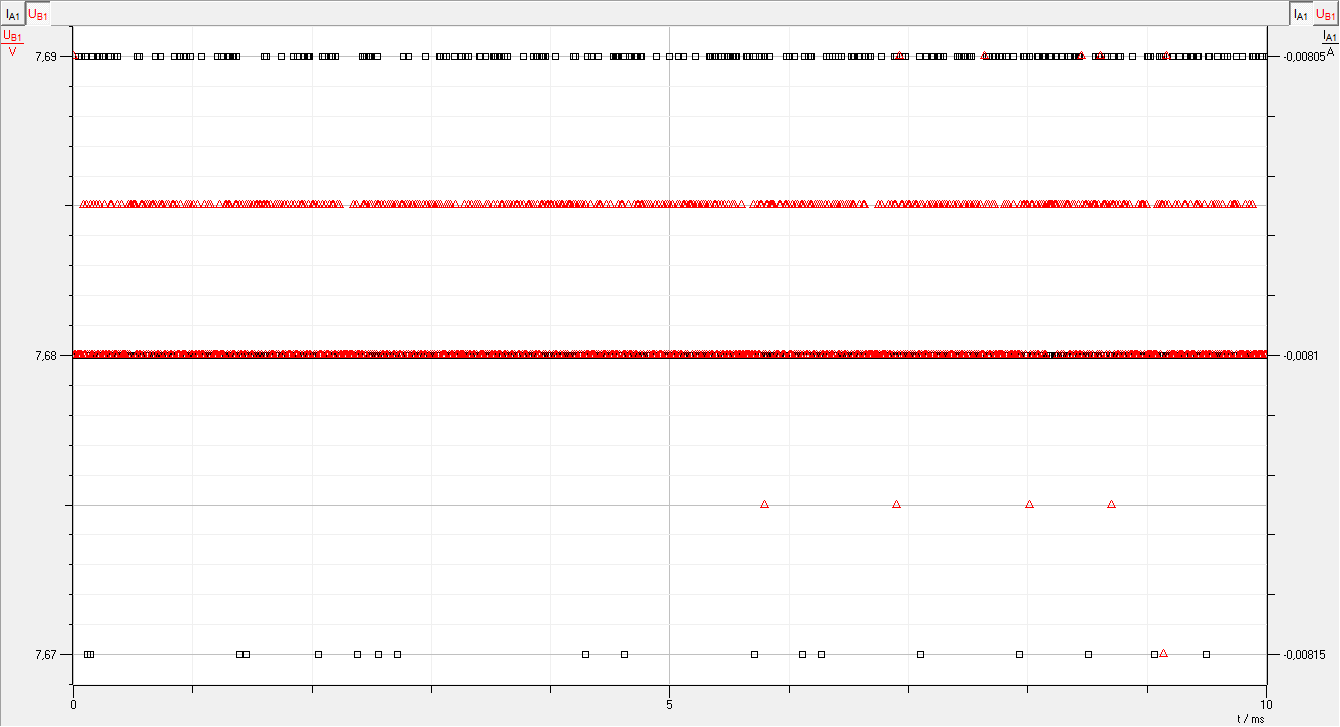
\includegraphics[scale=0.575]{Rauschmessung2.png}  
\caption{Rauschmessungen}
\end{figure}
\newpage
\subsubsection{Analyse}
%Analyse der Daten inklusive Fehlerrechnung Residuen und Pullverteilung. (1 Seite)
Formeln:
\begin{align*}
R=\frac{\bar{U}}{\bar{I}} \hspace{2cm} 
\sigma_R=\sqrt{(\frac{1}{\bar{I}})^{2} \cdot \sigma_{\bar{U}}^{2}+(\frac{\bar{U}}{\bar{I}^2})^{2} \cdot \sigma_{\bar{I}}^{2}} \hspace{2cm}\frac{\sigma_R}{R}=\sqrt{(\frac{\sigma_{\bar{U}}}{\bar{U}})^2+(\frac{\sigma_{\bar{I}}}{\bar{I}})^2}
\end{align*}
Aus den Fehlerrechnungen der statistischen Fehlern aus der Messung und den systematischen Fehlern aus den Herstellerangaben des Sensor-Cassy berechneten wir folgende Werte für R:
\begin{table}[H]\centering
\caption{1. Messung}
\begin{tabular}{c|c|c|c|c|c|c}
$\bar{U}$& $\sigma_{\bar{U}}$& $\bar{I}$& $\sigma_{\bar{I}}$& $R$& $\Delta R_{stat}$& $\Delta R_{sys}$ \\ \hline
$1.71V$& $0.00009V$& $0.002A$& $0.00002A$& $855\Omega$& $8.55\Omega$& $233.27\Omega$\\ 
$3.88V$& $0.00008V$& $0.004A$& $0.00002A$& $970\Omega$& $4.85\Omega$& $135.8\Omega$\\ 
$5.82V$& $0.00007V$& $0.006A$& $0.00003A$& $970\Omega$& $4.85\Omega$& $101.84\Omega$ \\
$7.68V$& $0.00009V$& $0.008A$& $0.000026A$& $960\Omega$& $2.4\Omega$& $74\Omega$ \\
\end{tabular} 
\end{table}
%\subsubsection{Fazit}
%Diskussion der Ergebnisse und Vergleich der erzielten Ergebnisse mit theoretischen %Vorhersagen.
\section{Charakterisierung des Widerstands}
\subsection{Versuchsbeschreibung}
Wie bereits im vorherigen Versuch, geht es in diesem Versuch um die Bestimmung des Ohmschen Widerstandes. In diesem Teil werden wir durch Einzelmessungen verschiedener Spannungen eine Lineare Regression durchführen. Durch die maximale Variation der systematischen Fehler der gemessenen Größen U (in V) und I (in A) erhalten wir zwei neue Geraden, die einen Korridor um den Fit bilden, mit dessen Hilfe man die systematischen Fehler des Widerstands R (in $\Omega$) abschätzen kann.\\
Hierzu werden benötigt:\\
Das Ohmsche Gesetz \\
$R = \frac{U}{I}$\\
\\
Fehlerfortpflanzung\\
$\sigma_{R sys} = \sqrt{(\frac{a_{max}}{2})^2+(\frac{a_{min}}{2})^2}$\\
\subsection{Versuchsaufbau und Durchführung}
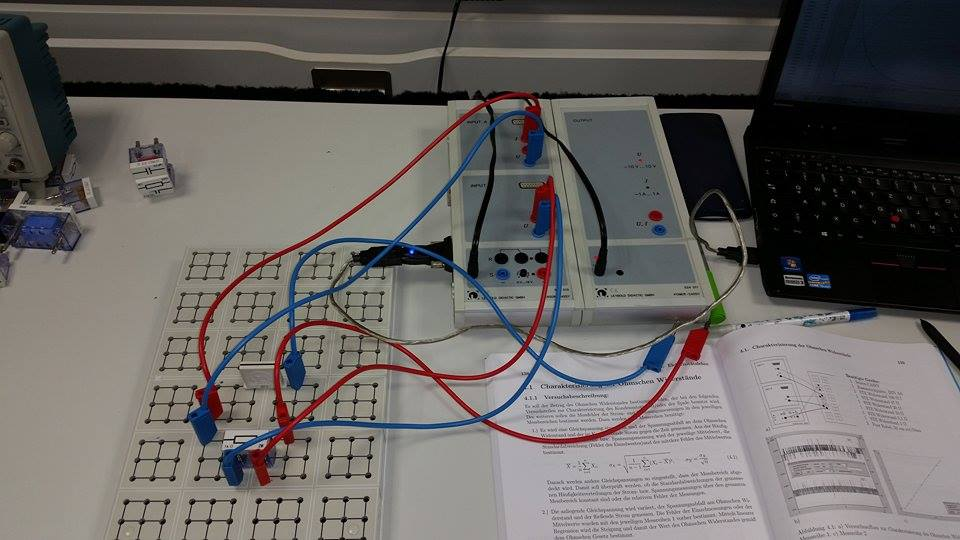
\includegraphics[scale=0.35]{12000155_1207085929316467_1534534399_n.jpg}\\
Der Aufbau unterscheidet sich nicht vom Aufbau der Rauschmessung. Wir wählen den gleichen Messbereich ($\pm$ 10V und $\pm$ 0.1A), stellen aber Cassy von automatischen Messungen auf Einzelmessungen um. Wir stellen verschiedene Spannungen ein (2V, 4V, 6V und 8V) und messen an den vorhandenen Punkten jeweils 4 mal (insgesamt 16 Messpunkte), um später einen möglichst genauen Fit zu bekommen. Wir verwenden den selben 1 k$\Omega$ Widerstand, wie im vorherigen Versuch, messen die Spannung parallel zum Widerstand und die Stromstärke in Reihe zwischen dem Widerstand und der Spannungsquelle.\\
\subsection{Versuchsauswertung}
\subsubsection{Rohdaten}
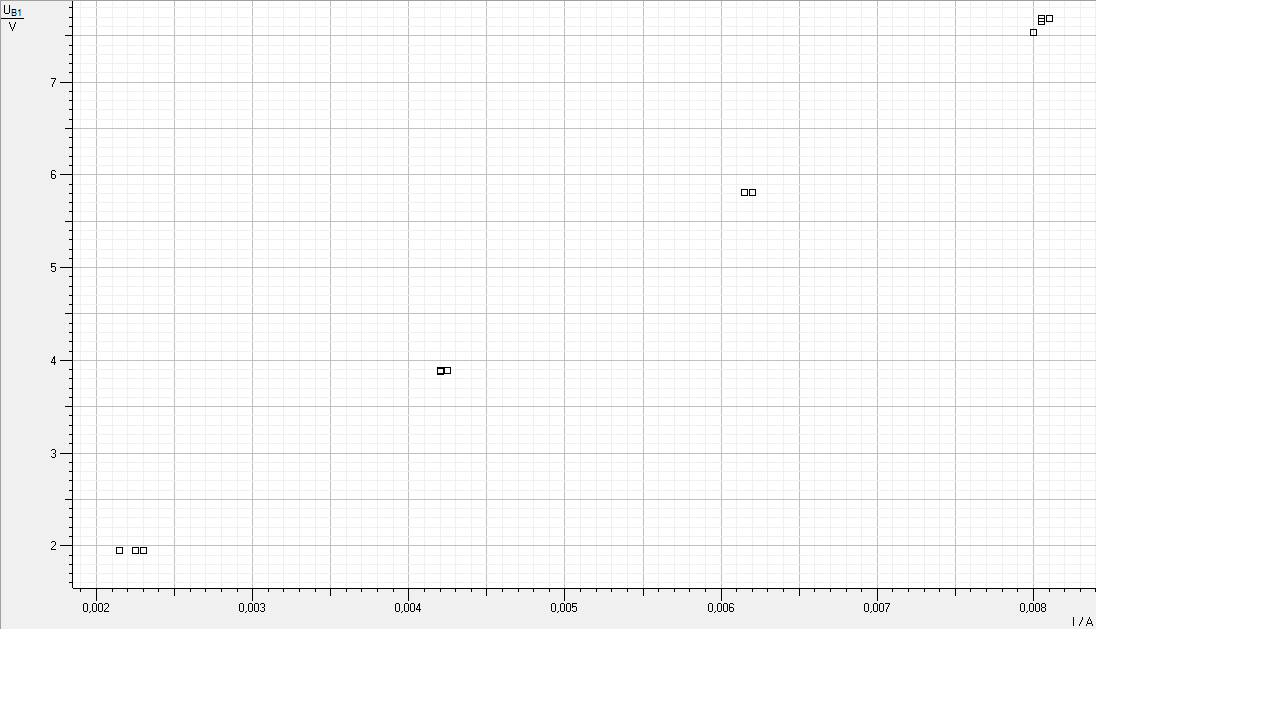
\includegraphics[scale=0.35]{raw_U_gegen_I.png}\\
\subsubsection{Transformation der Rohdaten}
Die oben gezeigten Rohdaten haben wir in Python eingelesen und anhand der in der Praktikumsbibliothek vorhandenen Routine zur Linearen Regression der Form $a\cdot x + b $ gefittet. Siehe:\\
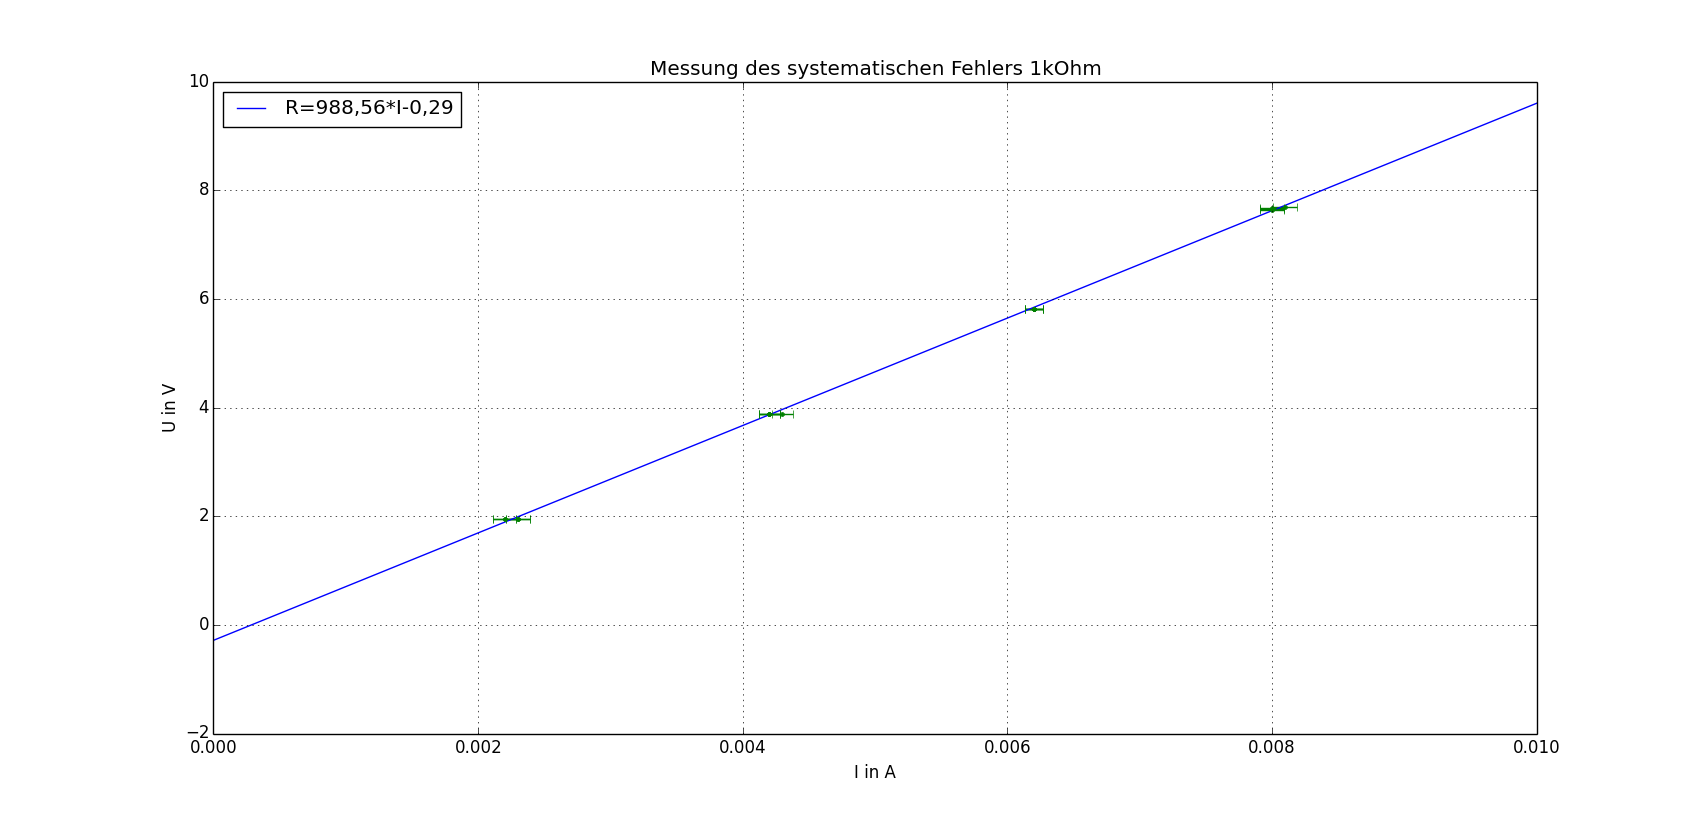
\includegraphics[scale=0.35]{lin_reg_single}
\\ In die Lineare Regression sind die statistischen Fehler auf die verschiedenen Spannungs- und Strombereiche eingegangen, die wir in der Rauschmessung vorher bestimmt hatten. Um den systematischen Fehler auf R abzuschätzen, müssen wir jetzt den "Korridor"$~$bilden. Dazu führen wir folgende Operationen aus.\\
\\$U_{i,verschoben} = U_i - (0.01 \cdot U_i + 0.005 \cdot 10V)$\\
$I_{i,verschoben} = I_i + (0.02 \cdot I_i + 0.005 \cdot 0.1A)$\\
\\bzw\\
\\$U_{i,verschoben} = U_i + (0.01 \cdot U_i + 0.005 \cdot 10V)$\\
$I_{i,verschoben} = I_i - (0.02 \cdot I_i + 0.005 \cdot 0.1A)$\\
\\Die sich so ergebenden zwei Geraden sehen wie folgt aus:\\
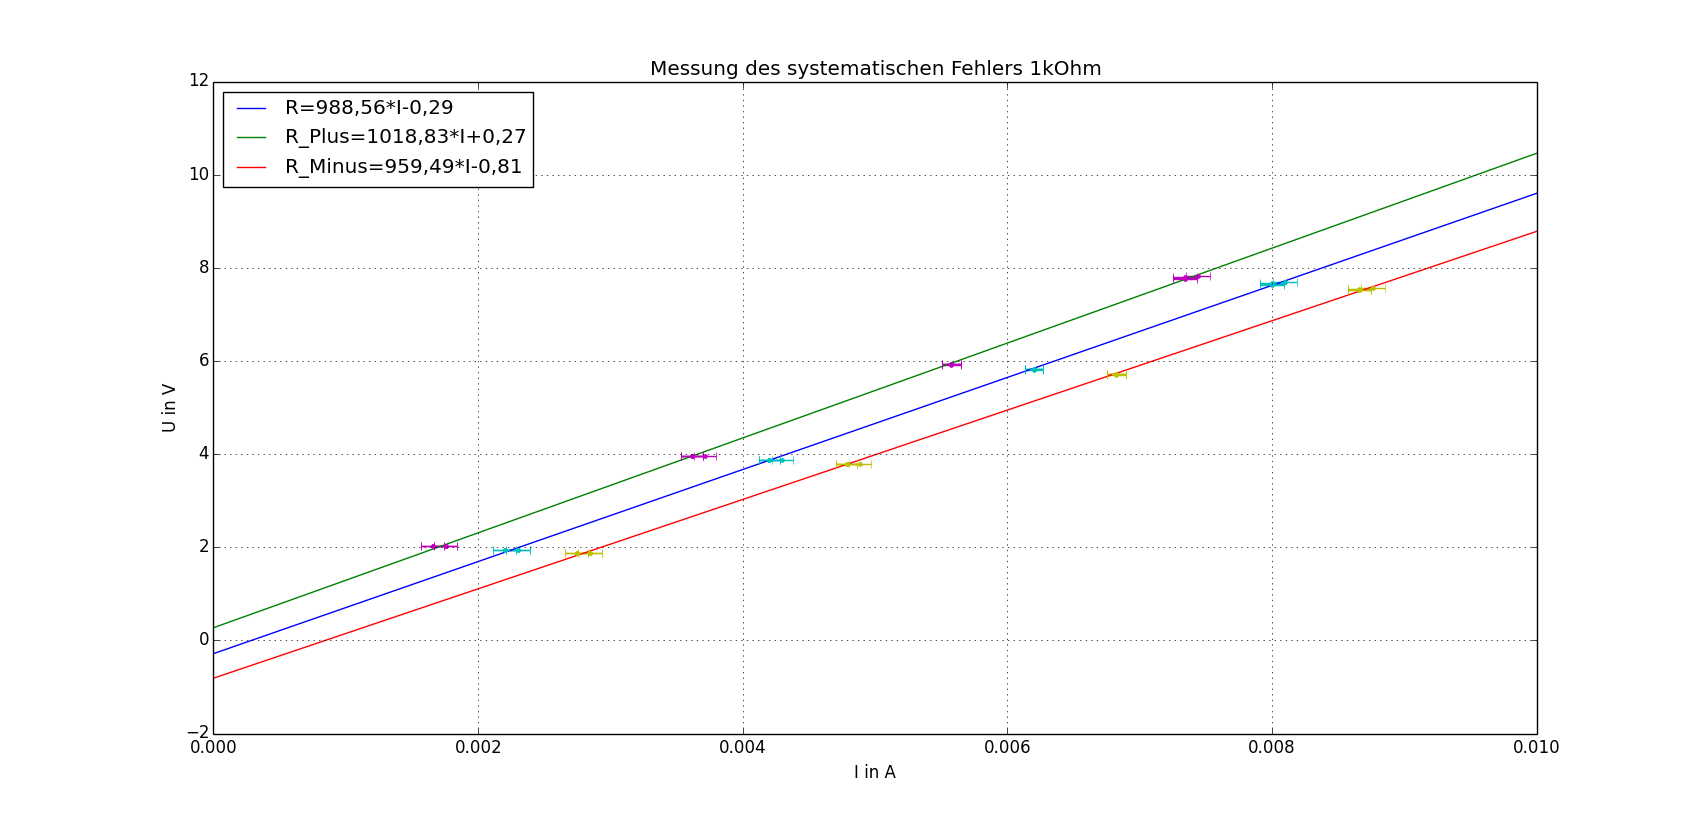
\includegraphics[scale=0.35]{U_gegen_I.png}
\\Zur Abschätzung des systematischen Fehlers ziehen wir die Steigung der minimalen Fitverschiebung von der Steigung der maximalen Fitverschiebung ab.\\  
$R_{sys} = a_{max} - a_{min}$\\
Der systematische Fehler beträgt nach unserer Abschätzung $\pm$ 59.337608$\Omega$.\\ 
Den Fehler darauf erhalten wir durch:\\
$\sigma_{R sys} = \sqrt{(\frac{a_{max}}{2})^2+(\frac{a_{min}}{2})^2}$\\
Der Fehler auf den systematischen Fehler beträgt $\pm$ 3.857496$\Omega$.\\
\\Aus den Werten der Rauschmessungen erhalten wir mit den Formeln zum gewichteten Mittelwert und dessen Fehlerfortpflanzung:\\
\\$\bar{R} = \frac{\sum{\frac{R}{(\sigma_{sys}+\sigma_{stat})^2}}}{\sum{\frac{1}{(\sigma_{sys}+\sigma_{stat})^2}}}$ und $\sigma_{R_{ges}} = \sqrt{\frac{1}{\sum{\frac{1}{(\sigma_{sys}+\sigma_{stat})^2}}}}$\\
\\Somit erhalten wir durch Einsetzen unserer Werte ein Endergebnis von 958.798$\Omega \pm$ 1.916 $\Omega_{stat} \pm$ 53.154 $\Omega_{sys}$\\
Unser Ergebnis für den systematischen Fehler liegt sehr nahe an unserer Abschätzung, daher vermuten wir, dass wir mit unserem Ergebnis richtig liegen.\\ 
\subsubsection{Fazit}
In der dritten Messreihe haben wir den Widerstand mit Hilfe eines Multimeters vermessen. Der Wert hierfür betrug $0.993 k\Omega \pm$ 1 $\Omega \pm$ 16 $\Omega$ + 3 ST. \\ 
\\Vergleichen wir unseren Wert (958.798$\Omega$) mit dem der Messreihe 3 unter Berücksichtung der Fehler, können wir guten Gewissens eine Übereinstimmung der Werte festhalten. 
\\Der Hersteller gibt 1k$\Omega$ mit einer Toleranz von $\pm$ 5\% an, sprich 0.950k$\Omega$ - 1.050k$\Omega$. 
\\Unser Wert stimmt auch hier sehr gut überein.  
\section{Auf- und Entladung eines Kondensators, Teilversuch 4.2}
\subsection{Versuchsbeschreibung}
\subsubsection*{Aufladung}
Das Ziel dieses Versuches ist es aus dem Strom- bzw. Spannungsverlauf beim Auf- bzw. Entladen des Kondesators die Zeitkonstante
\[\tau = R \cdot C \]
der nachfolgenden Schaltung zu bestimmen.
Nach Kirchhoff gilt in diesem Fall:
\begin{align*}
U_0-U_R(t)-U_C(t)=0 \rightarrow U_0-U_C(t)=I(t) \cdot R
\end{align*}
Nach Aufstellen und Lösen der DGL's ergeben sich für die Aufladung die Gleichungen:
\begin{align*}
U_C(t)=U_0 \cdot (1-e^{-\frac{t}{R \cdot C}}) \hspace{2cm} I(t)=I_0 \cdot e^{-\frac{t}{R \cdot C}}
\end{align*}
Aus denen sich nun $\tau=R \cdot C$ berechnen lässt.
\subsubsection*{Entladung}
Wird der Schalter nun geschlossen liefert uns die Maschenregel:
\begin{align*}
R \cdot I(t) + U_C(t) = 0
\end{align*}
Aufstellen und Lösen der DGL ergibt dann in diesem Fall:
\begin{align*}
U_C(t)=U_0 \cdot e^{-\frac{t}{\tau}} \hspace{2cm} I(t)=-\frac{U_0}{R} \cdot e^{-\frac{t}{\tau}}
\end{align*}
\subsection{Versuchsaufbau und Durchführung}
\begin{center}
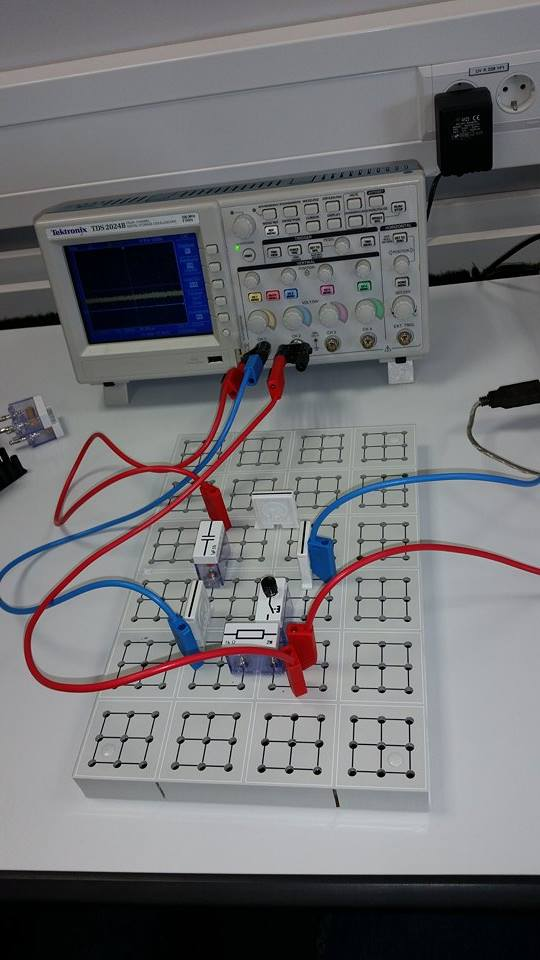
\includegraphics[scale=0.6]{12834525_1207198235971903_753892727_n.jpg}
\end{center}
Wie man im obigen Bild sieht besteht unser Versuchsaufbau aus einem in Reihe geschalteten Kondensator und einem Widerstand. Mit dem Oszilloskop wird dann auf Channel 1 die Spannung am Kondensator und auf Channel 2 der Strom gemessen. Dafür wurden die Channel geerdet.
Die Spannungsquelle kann mittels Schalter überbrückt werden, um die Entladung des Kondensators einzuleiten.
Für die Messungen wurden jeweils 1000 Werte in einem Messzeitraum von 10$ms$ aufgezeichnet. Der Messbereich der Spannung lag zwischen $-10V$ und $+10V$, die des Stroms zwischen $-0,1A$ und $+0,1A$.
Der Trigger des Oszilloskop wurde für die Aufladung auf $360mV$ aufsteigend, für die Entladung auf $1,76V$ absteigend eingestellt.
\subsection{Versuchsauswertung}
Nachdem zunächst aus den Daten die Offsests von $80mA$ bzw. $80mV$ korrigiert wurden, ergeben sich mit:
\begin{align*}
\frac{U_1}{U_2}=e^{-\frac{t_1-t_2}{\tau}}
\end{align*}
die Formeln:
\begin{align*}
\tau=\frac{\Delta t}{\ln{\frac{U_1}{U_2}}} \hspace{2cm}
\sigma_{\tau}=\sqrt{(\frac{\sigma_{\Delta t}}{\ln{\frac{U_1}{U_2}}})^2+(\frac{\Delta t}{U_1} \cdot \sigma_{U_1})^2+(-\frac{\Delta t}{U_2} \cdot \sigma_{U_2})^2}
\end{align*}
aus denen wir dann später die Kapazität C und dessen statistischen Fehler $\sigma_C$ bestimmen können.
Der systematische Fehler wurde durch die Korrektur des Offsets auf den systematischen Fehler auf $R$ reduziert. Dieser ergibt sich dann aus:
\begin{align*}
\frac{\sigma_{C,sys}^R}{C}=\frac{\sigma_{R,sys}}{R}
\end{align*}
\subsubsection{Rohdaten}
Mithilfe des Cursers des Oszilloskops wurden die Spannungen bzw. Ströme mit einem Abstand von $1ms$ abgelesen und ein Ablesefehler von $0,04mA$,      \hspace{1mm} $0,04V$ und $0,04ms$ notiert und anschließend durch $\sqrt{12}$ geteilt um die Gleichverteilung zu berücksichtigen.
\begin{table}[H]\centering
\caption{Oszilloskop}
\begin{tabular}{c|c}
$I_1$& $I_2$\\ \hline
$0,72A$& $1,88A$\\ 
$0,8A$& $2,24A$ \\
$0,76A$& $2,12A$ \\
$0,72A$& $1,92A$ \\
\\
$U_1$& $U_2$ \\ \hline
$0,84V$& $2,48V$ \\
$0,84V$& $2,44V$ \\
$0,80V$& $2,40V$ \\
$0,89V$& $2,44V$ \\
\end{tabular} 
\end{table}
\subsubsection{Analyse/Transformation der Rohdaten}
Aus den Werten der Auf- und Entladung wurden anschließend jeweils $\tau$ und $\sigma_{\tau}$ berechnet und mithilfe von:
\begin{align*}
C=\frac{\tau}{R} \hspace{2cm} \sigma_C=\sqrt{(\frac{\sigma_{\tau}}{R})^2+(-\frac{\tau}{R^2}\cdot \sigma_R)^2}
\end{align*}
wurden dann die Kapazitäten und ihre statistischen Fehler berechnet.
Danach haben wir dann aus den Ergebnissen den gewichteten Mittelwert und dessen Fehler berechnet. Der systematische Fehler wurde dabei aus den Ergebnissen der Widerstandsmessung berechnet.
Zu guter Letzt haben wir die Einzelergebnisse mit ihren Gesamtfehlern zusammen mit unserem Mittelwert geplottet.
\begin{figure}[hbtp]
\centering
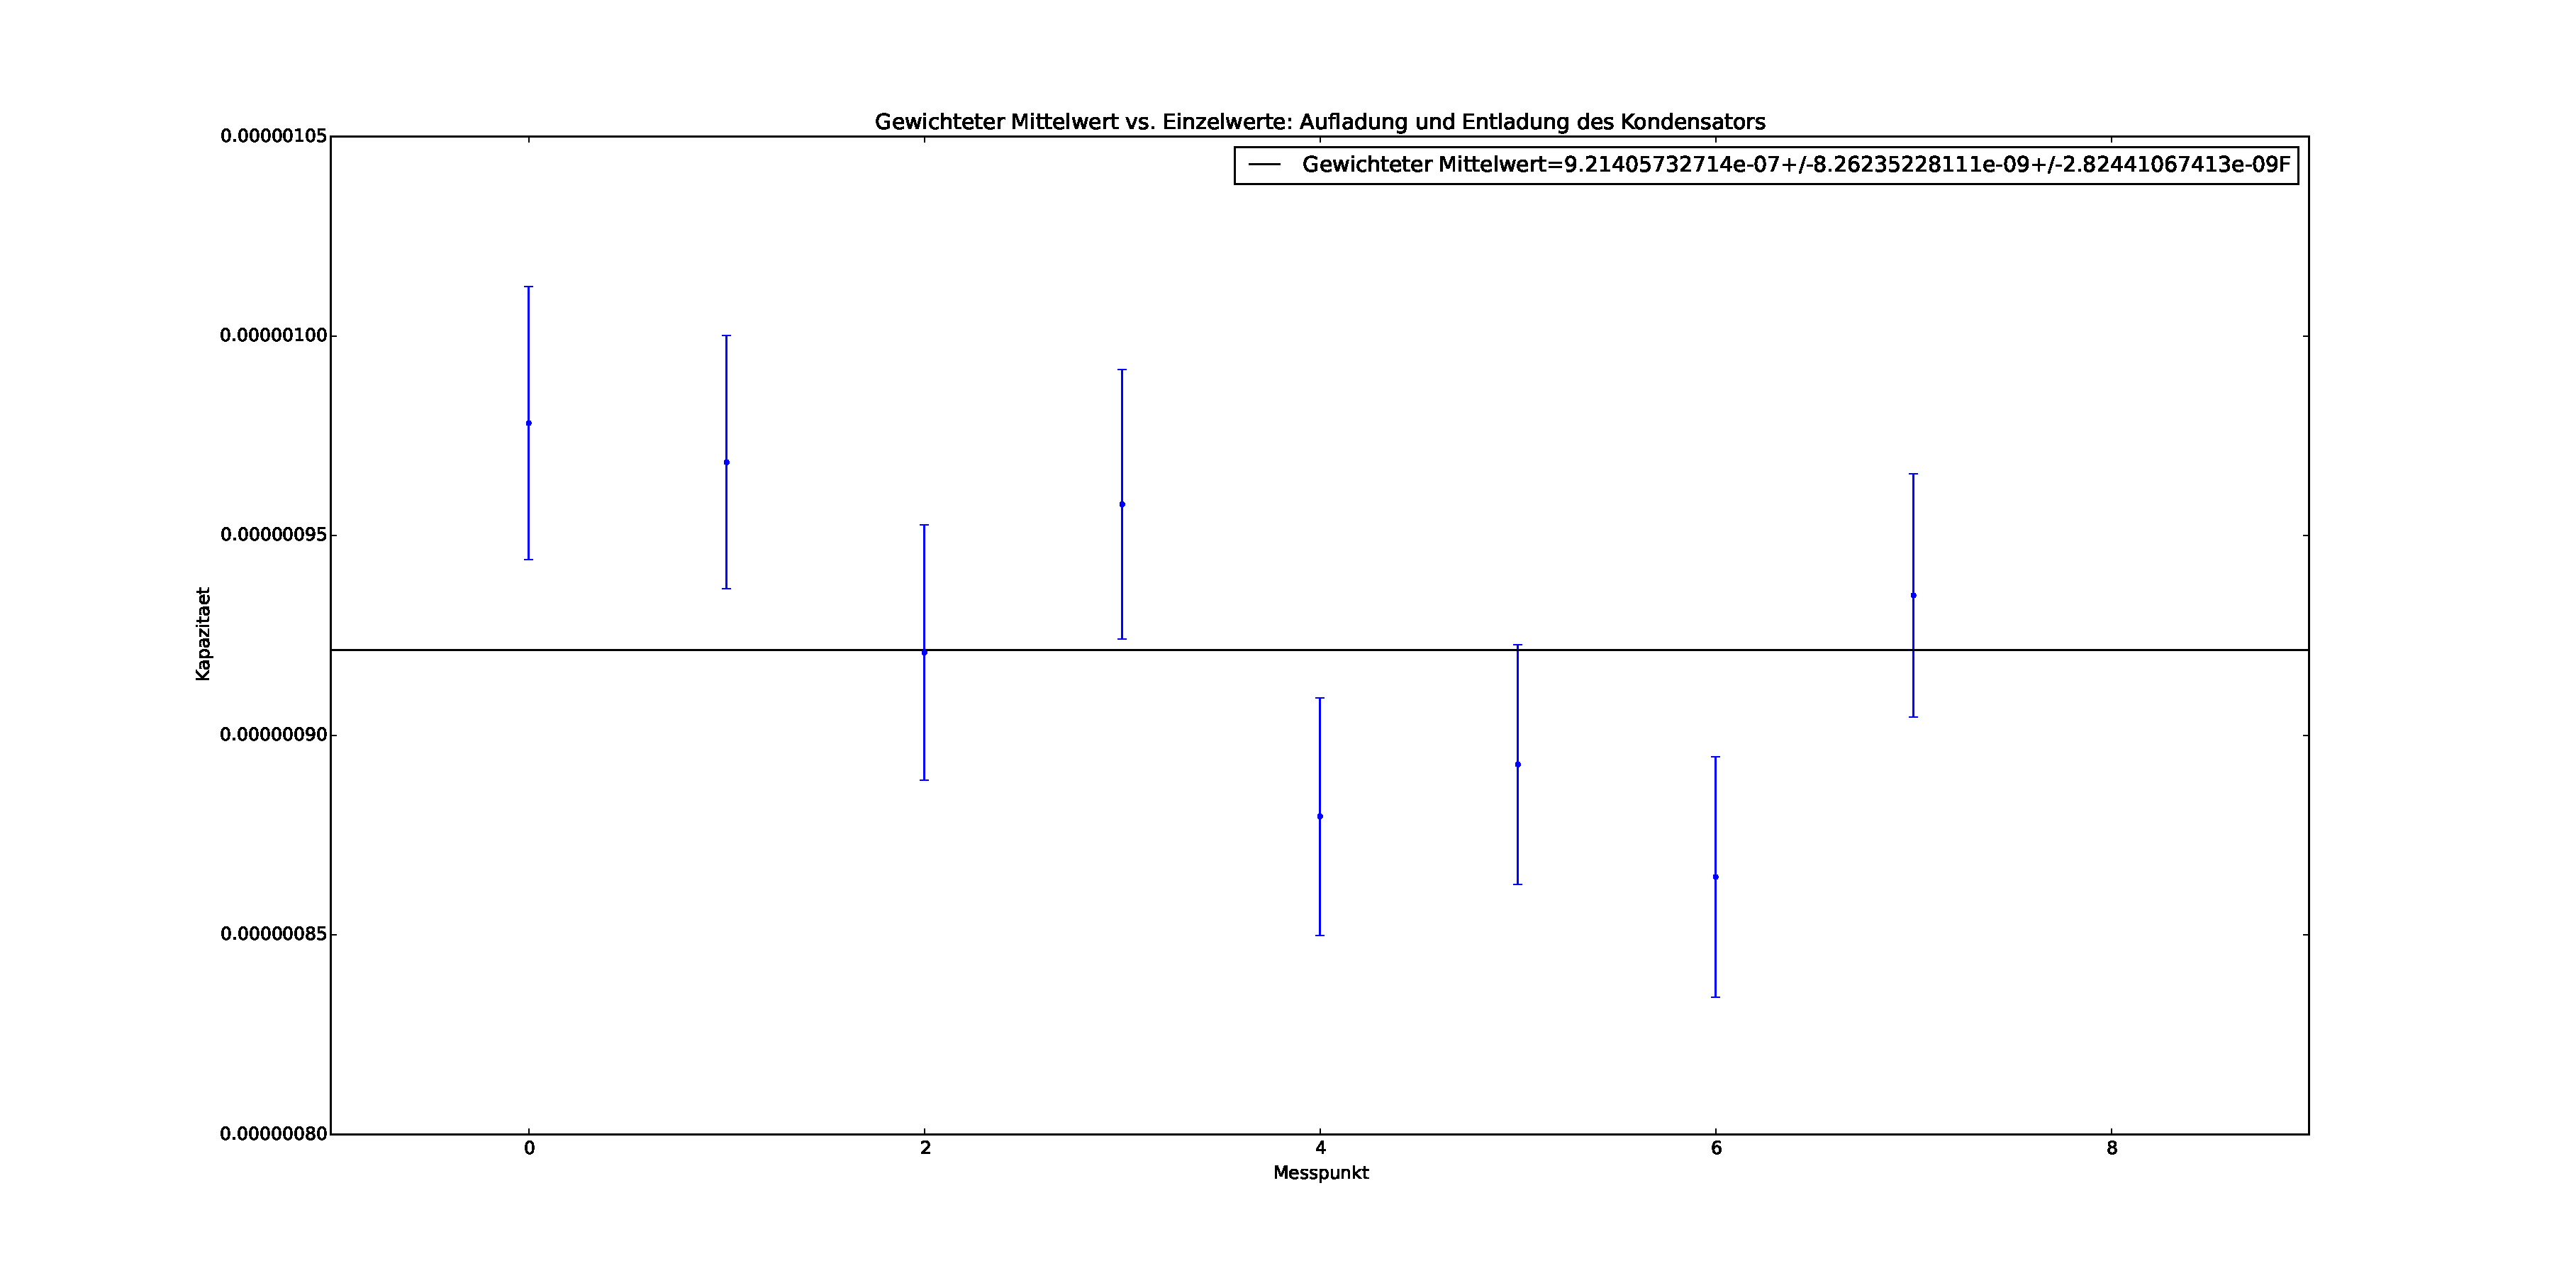
\includegraphics[scale=0.3]{auf-entladung.eps}
\caption{Ergebnisse vs. Mittelwert}
\end{figure}
\subsubsection{Fazit}
Aus den Ergebnissen der Analyse zeigt sich, dass drei der Werte für $C$ mit $1\sigma$ Abweichung und alle Werte mit $2\sigma$ Abweichung im Bereich des Mittelwerts liegen. Die etwas zu große Abweichung des Endergebnisses vom Literaturwerts von $1\mu F$ mit einer Toleranz von $5 \%$, lässt sich durch nicht berücksichtigte systematische Fehler wie z.B. ein größerer Widerstand, bedingt durch die verwendeten Kabel und Steckplattenbauteile, erklären.
\section{Charakterisieren eines Kondensators}
\subsection{Versuchsbeschreibung}
In diesem Teil des Versuchs werden wir uns im speziellen die Lade- bzw. Entladekurven des Kondensators anschauen, um diesen zu bestimmen. Wir werden danach in Python die Daten auswerten, logarithmisch fitten und so beim Aufladevorgang die Kapazität C (in $\mu$F) über den Verlauf der Stromstärke, sowie beim Entladevorgang über den Spannungsverlauf bestimmen. Wir werden unsere Ergebnisse anhand von Residuenplots evaluieren.\\
\subsection{Versuchsaufbau und Durchführung}
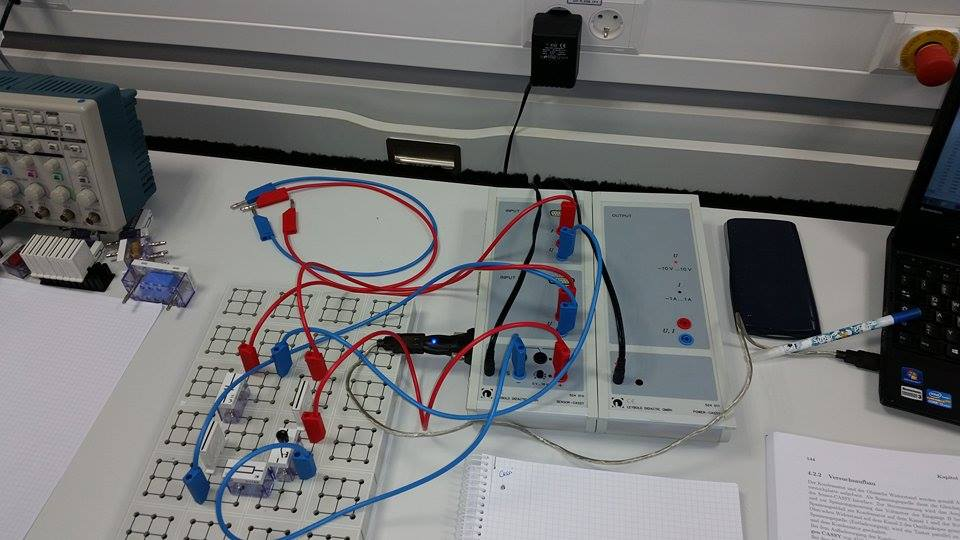
\includegraphics[scale=0.35]{12834837_1207198225971904_686312351_n.jpg}
\\Oben sieht man unseren Versuchsaufbau. Dieser unterscheidet sich prinzipiell nicht vom Aufbau bei der Messung mit dem Oszilloskop. Wir greifen immer noch parallel zum Kondensator die Spannung ab, sowie in Reihe die Stromstärke. Ein Schalter unterbricht den Stromkreis und löst so den Lade- bzw. Entladevorgang aus.\\
\\Unser Messbereich im Cassy liegt für die Spannung bei 10V und bei der Stromstärke 0.1A. Wir verwenden einen 1k$\Omega$ Widerstand um den Lade- und Entladevorgang zu verzögern. Des Weiteren verwenden wir einen 1$\mu$F Kondensator den wir im Experiment charakterisieren möchten.\\
Als Trigger benutzen wir die eingebaute Cassy-Funktion und triggern jeweils die Spannung (0.4V beim Ladevorgang, 7.6V beim Entladevorgang).\\
Wir verwenden die höchstmögliche Messauflösung von 10$\mu$s und 10ms Messzeit.\\
\\Beim Ladevorgang stellen wir die automatische Umschaltfunktion der Spannungsquelle (8V Ladespannung) des Cassy an und starten dann die Messung. Wir messen sowohl die Stromstärke, als auch die Spannung, betrachten aber später aufgrund ihrer Form beim Ladevorgang nur den Verlauf der Stromstärke. Wir messen insgesamt 4 Ladevorgänge, um später den Kondensator genauer bestimmen zu können. \\
\\Beim Entladevorgang schalten wir die Spannungsquelle von vornherein an, warten ab bis sich die Ladespannung von 8V eingestellt hat und triggern jetzt den Abfall der Spannung. Den Trigger lösen wir durch kurzschließen der Spannungsquelle aus. Der dabei gemessene Spannungsverlauf wird dann später ausgewertet. Auch hier messen wir wieder 4 mal, um unsere Genauigkeit zu erhöhen.\\
\subsection{Versuchsauswertung}
\subsubsection{Rohdaten}
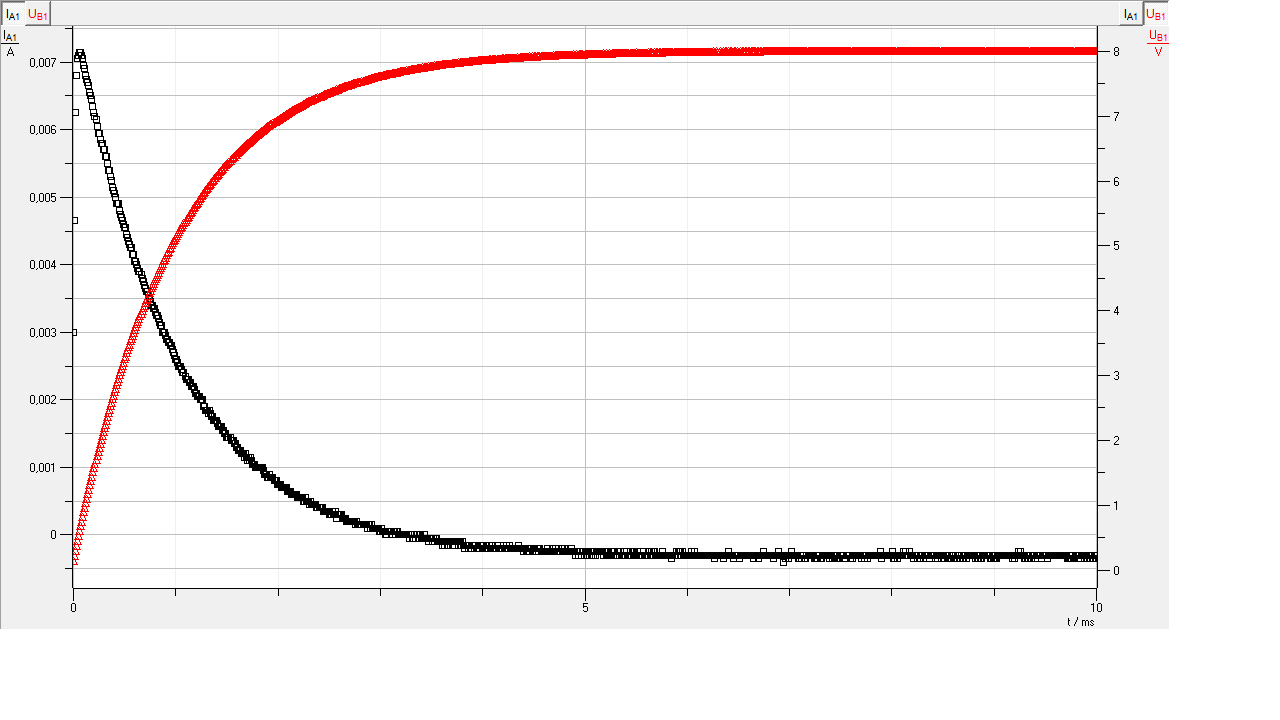
\includegraphics[scale=0.35]{auf1.png}\\
Aufladevorgang (U in V [rot], I in A [schwarz]gegen t in ms)\\
\\
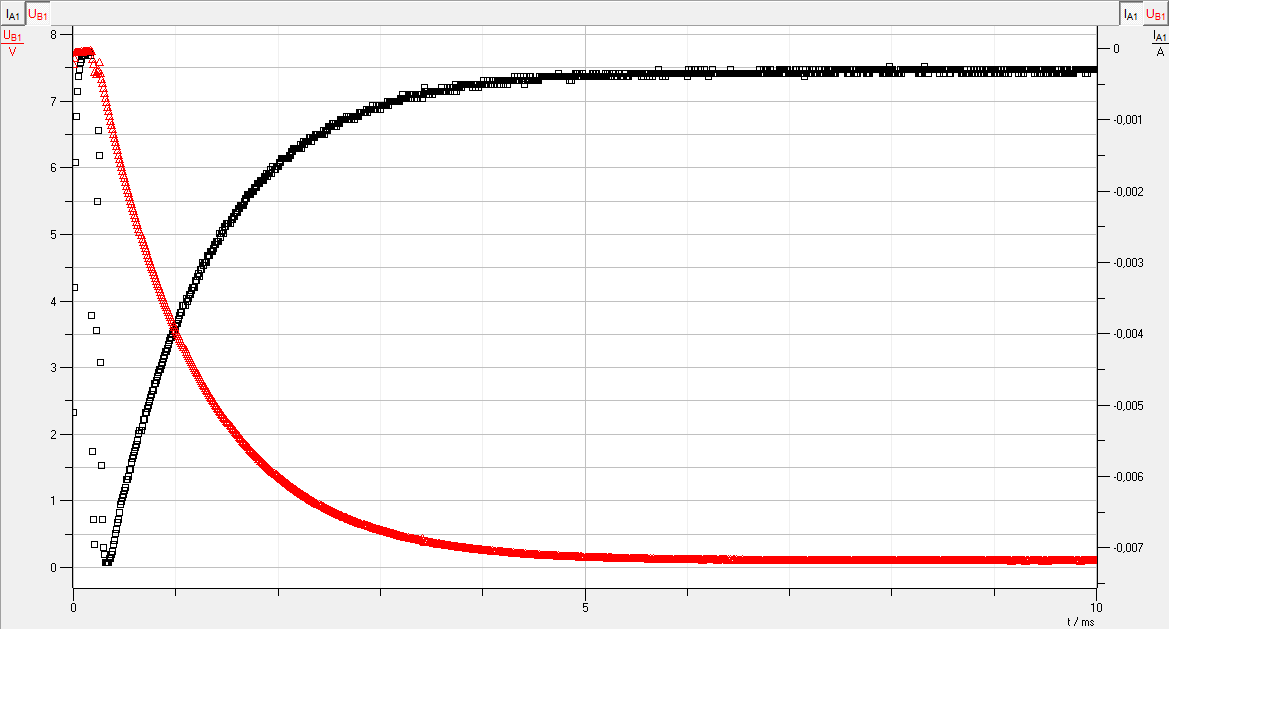
\includegraphics[scale=0.35]{ent1.png}\\
Entladevorgang (U in V [rot], I in A [schwarz]gegen t in ms)\\

\subsubsection{Transformation der Rohdaten}
Um an den oben aufgeführten Daten eine Lineare Regression durchführen zu können müssen wir die Datenpunkte logarithmieren. Wie bereits vorher angekündigt verwenden wir beim Ladevorgang nur die Daten der Stromstärkenmessung und beim Entladevorgang die Daten der Spannungsmessung. Im Folgenden werden wir das jeweils anhand eines Beispieles für Spannung und Stromstärke zeigen, da der Bericht sonst zu lang wird. In unseren Endwerten sind alle Daten mit eingearbeitet, um ein möglichst genaues Ergebnis zu erzielen.\\
\\Bevor wir anfangen die Daten zu logarithmieren, müssen wir die Offsets bestimmen. Dies machen wir grafisch in Cassy.\\
Dazu zoomen wir auf den $\,$geraden$\,$ Bereich der abfallenden e-Funktion am Ende der Messung. Wenn wir nur noch Rauschen und keinen signifikanten Abfall der Werte sehen, können wir den untersten Peak mit einer Einheit in der Größenordnung darunter als Offset bestimmen. In dieser Ansicht können wir auch die Auflösung der Spannung bzw. Stromstärke ablesen, aus der wir die gleichverteilte Unsicherheit auf unsere Messwerte ablesen. Wir verfahren ähnlich mit der Zeitskala und bei den anderen Messungen.\\
\\
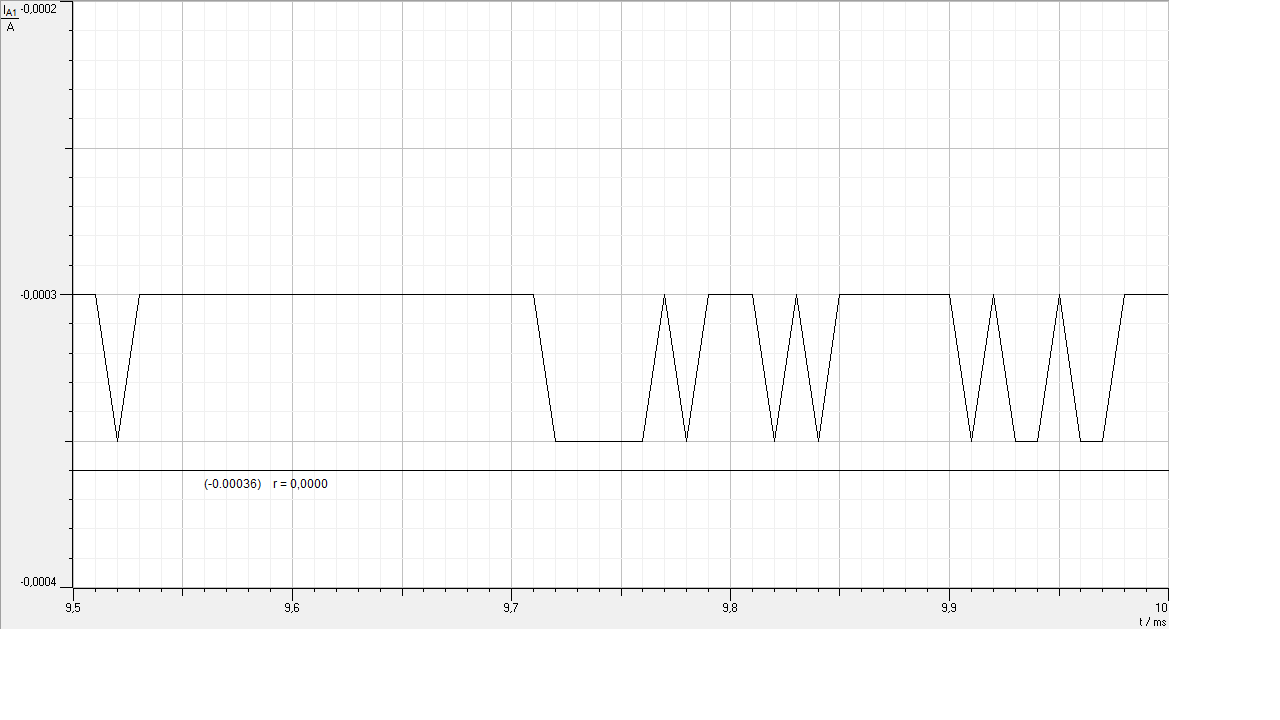
\includegraphics[scale=0.35]{offset_und_fehler.png}\\
Unterer Bereich des Ladevorgangs (I in A gegen t in ms) und Offsetmarkierung\\
\\
\\In unserem Beispiel haben wir nun einen Offset bei der Aufladung von -0.00041 A, einen Fehler auf I von $\frac{0.00005}{\sqrt{12}}$A und einen Fehler auf t von $\frac{0.01\cdot10^{-3}}{\sqrt{12}}$ms (die $\sqrt{12}$ ergeben sich aus der Gleichverteilung der Ablesefehler). Beim Entladevorgang verfahren wir analog und haben einen Offset von 0.079V, sowie einen Fehler auf U von $\frac{0.005}{\sqrt{12}}$V und einen Fehler auf t von $\frac{0.01\cdot10^{-3}}{\sqrt{12}}$.ms\\
\\Nachdem wir die Offsets korrigiert haben, können wir gefahrlos den Logarithmus ausführen (vorher liefen wir vor allem beim negativen Offset der Stromstärke Gefahr ein negatives Argument im Logarithmus zu haben, das hätte zu einer Anomalie geführt, mit der wir keine Lineare Regression hätten durchführen können). Die Daten sehen nun wie folgt aus: \\
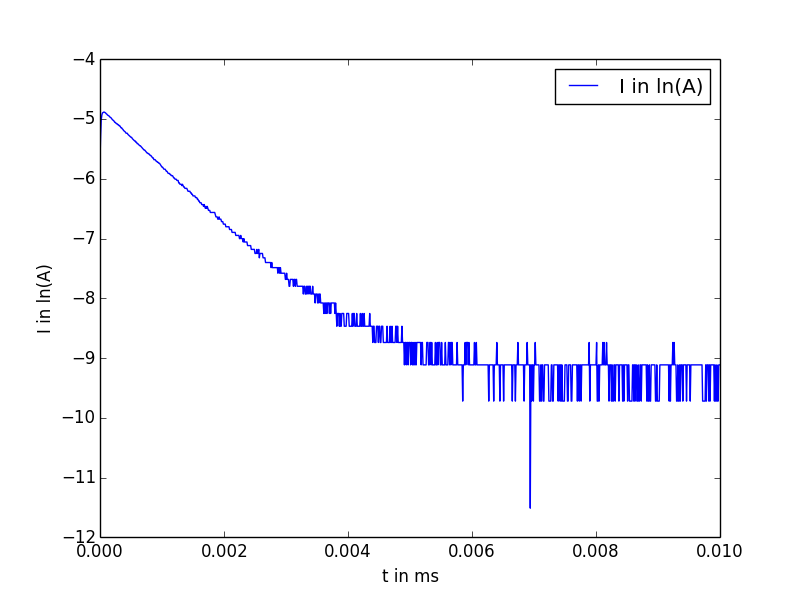
\includegraphics[scale=0.35]{ln(I)ggt.png}\\
Logarithmierter I-Datensatz (Einheiten siehe Grafik)\\
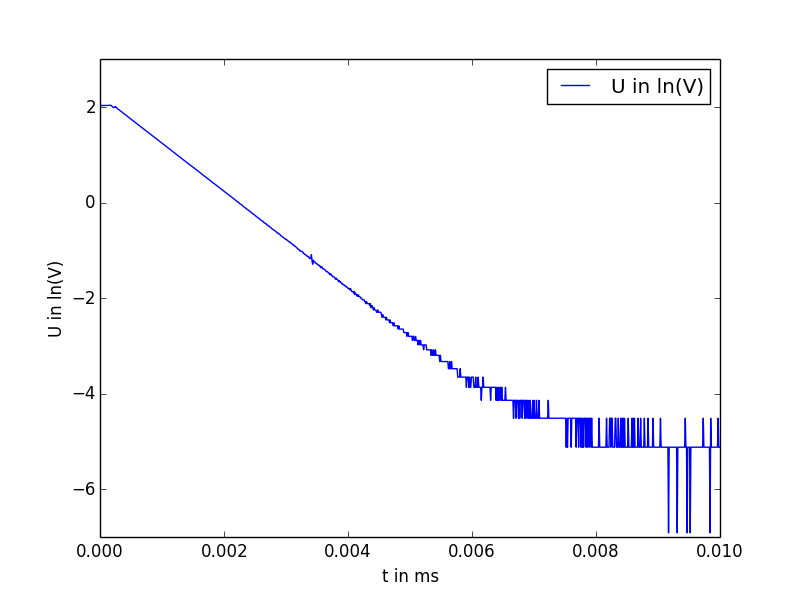
\includegraphics[scale=0.35]{ln(u)ggt.png}\\
Logarithmierter U-Datensatz (Einheiten siehe Grafik)\\
\\ Wir erkennen eindeutig am Anfang und Ende unserer Daten Bereiche, die in einer Lineare Regression unser Ergebnis deutlich verfälschen würden. Wir werden daher nur Datenpunkte nehmen, die einer Geraden auf der logarithmischen Skala entsprechen.
Nun sehen unsere Daten wie folgt aus:\\
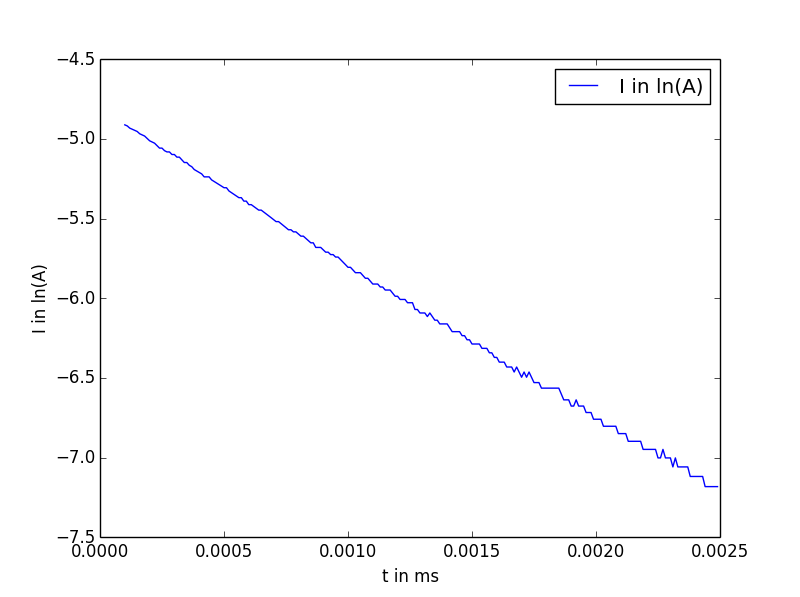
\includegraphics[scale=0.35]{ln(Ik)ggt.png}\\
Logarithmierter I-Datensatz mit angepasstem Bereich(Einheiten siehe Grafik)\\
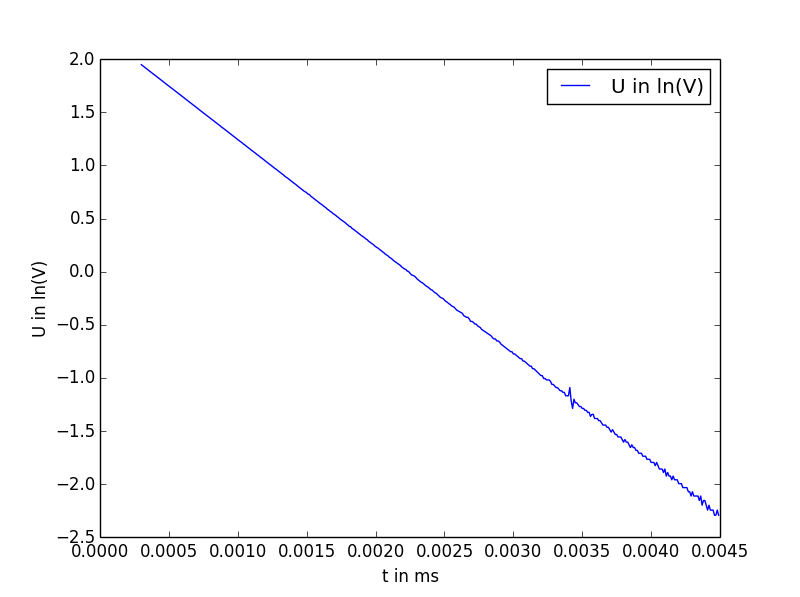
\includegraphics[scale=0.35]{ln(uk)ggt.png}\\
Logarithmierter U-Datensatz mit angepasstem Bereich(Einheiten siehe Grafik)\\
\\Jetzt führen wir die Lineare Regression durch.\\
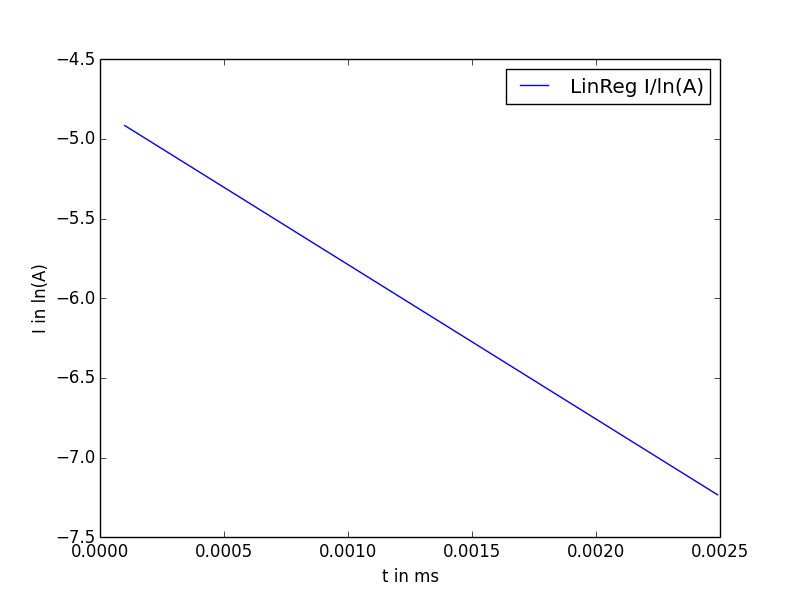
\includegraphics[scale=0.35]{lin_reg_I}\\
\\$\chi^2 = 3.046431$\\
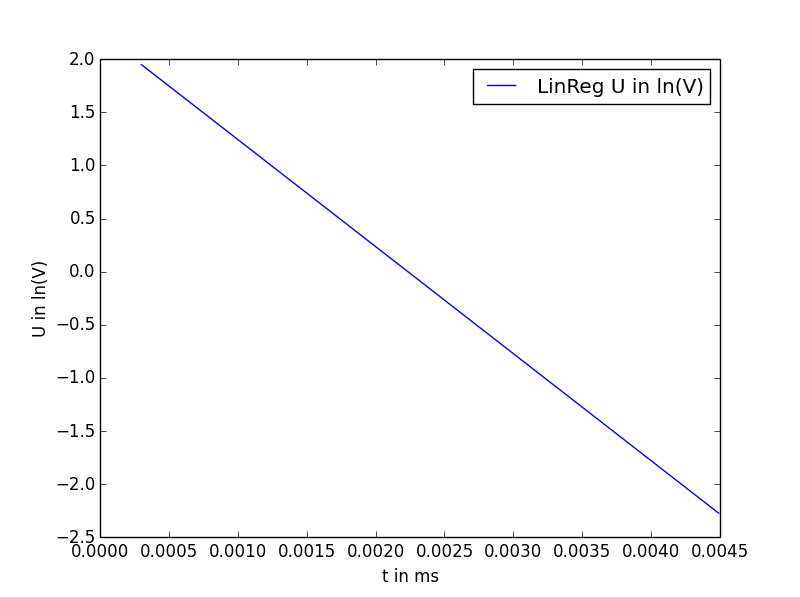
\includegraphics[scale=0.35]{lin_reg_U}\\
\\$\chi^2 = 2.469800$\\
\\Der Fehler pflanzt sich wie folgt fort:\\
\\$\sigma_{LinReg} = \frac{\sigma_I}{I}$\\
\\Um die Unsicherheit auf U zu bestimmen verfahren wir genauso wie bei I.\\
Die Lineare Regression hat die Form a$\cdot x + $b. Wie im Skript erläutert können wir nun aus unserem vorher bestimmten Widerstand (siehe Versuch 1) und der Steigung der Geraden die Kapazität ausrechnen.\\
\\$C = -\frac{1}{a\cdot R}$\\
\\Daraus ergibt sich die statistische Unsicherheit auf C von:\\
\\$\sigma_C = \sqrt{(\frac{\sigma_a}{a})^2+(\frac{\sigma_R}{R})^2}\cdot C$\\
\\Wir prüfen anhand der Residuenverteilungen, ob die Offset-Korrektur ausreichend war. Das Residuum erhalten wir, indem wir die Differenz von unseren Daten und dem Fit bilden. Die Fehler werden wie üblich fortgepflanzt.\\
\\$Residuum = I - LinReg(I)$\\
Analog dazu U.\\
\\$\sigma_{Residuum} = \sqrt{(\sigma_{I})^2+(\sigma_{LinReg})^2}$\\
Das sollte uns gleichverteilte Werte als Streuung um 0 zurückgeben.\\
\includegraphics[scale=0.35]{residuum_I}\\
Residuum für I 
\includegraphics[scale=0.35]{residuum_U}\\
Residuum für U
\\Man erkennt eine $sin^2$-Systematik im Residuum für I, dies führen wir auf unsere unstete Spannungsquelle zurück. In den unbearbeiteten Cassy-Daten sieht man, dass sich die Spannungsquelle unregelmäßig an- und ausstellt. Das Residuum für U ist größtenteils gleichverteilt, streut aber am Ende auch mit einer $sin^2$ Charakteristik. Unser $\chi^2$ von 3.0 bzw 2,5 ist allerdings zufriedenstellend.\\
\\Danach pflanzen wir den systematischen Fehler fort:\\
\\$\sigma_{c_{sys}} = \frac{1}{a\cdot R^2}\cdot\sigma_{R_{sys}}$\\
\\Danach wiederholen wir alles für die restlichen Messungen und bilden den gewichteten Mittelwert:\\
\\$\bar{C} = \frac{\sum{\frac{C}{(\sigma_{sys}+\sigma_{stat})^2}}}{\sum{\frac{1}{(\sigma_{sys}+\sigma_{stat})^2}}}$ und $\sigma_{C_{ges}} = \sqrt{\frac{1}{\sum{\frac{1}{(\sigma_{sys}+\sigma_{stat})^2}}}}$\\
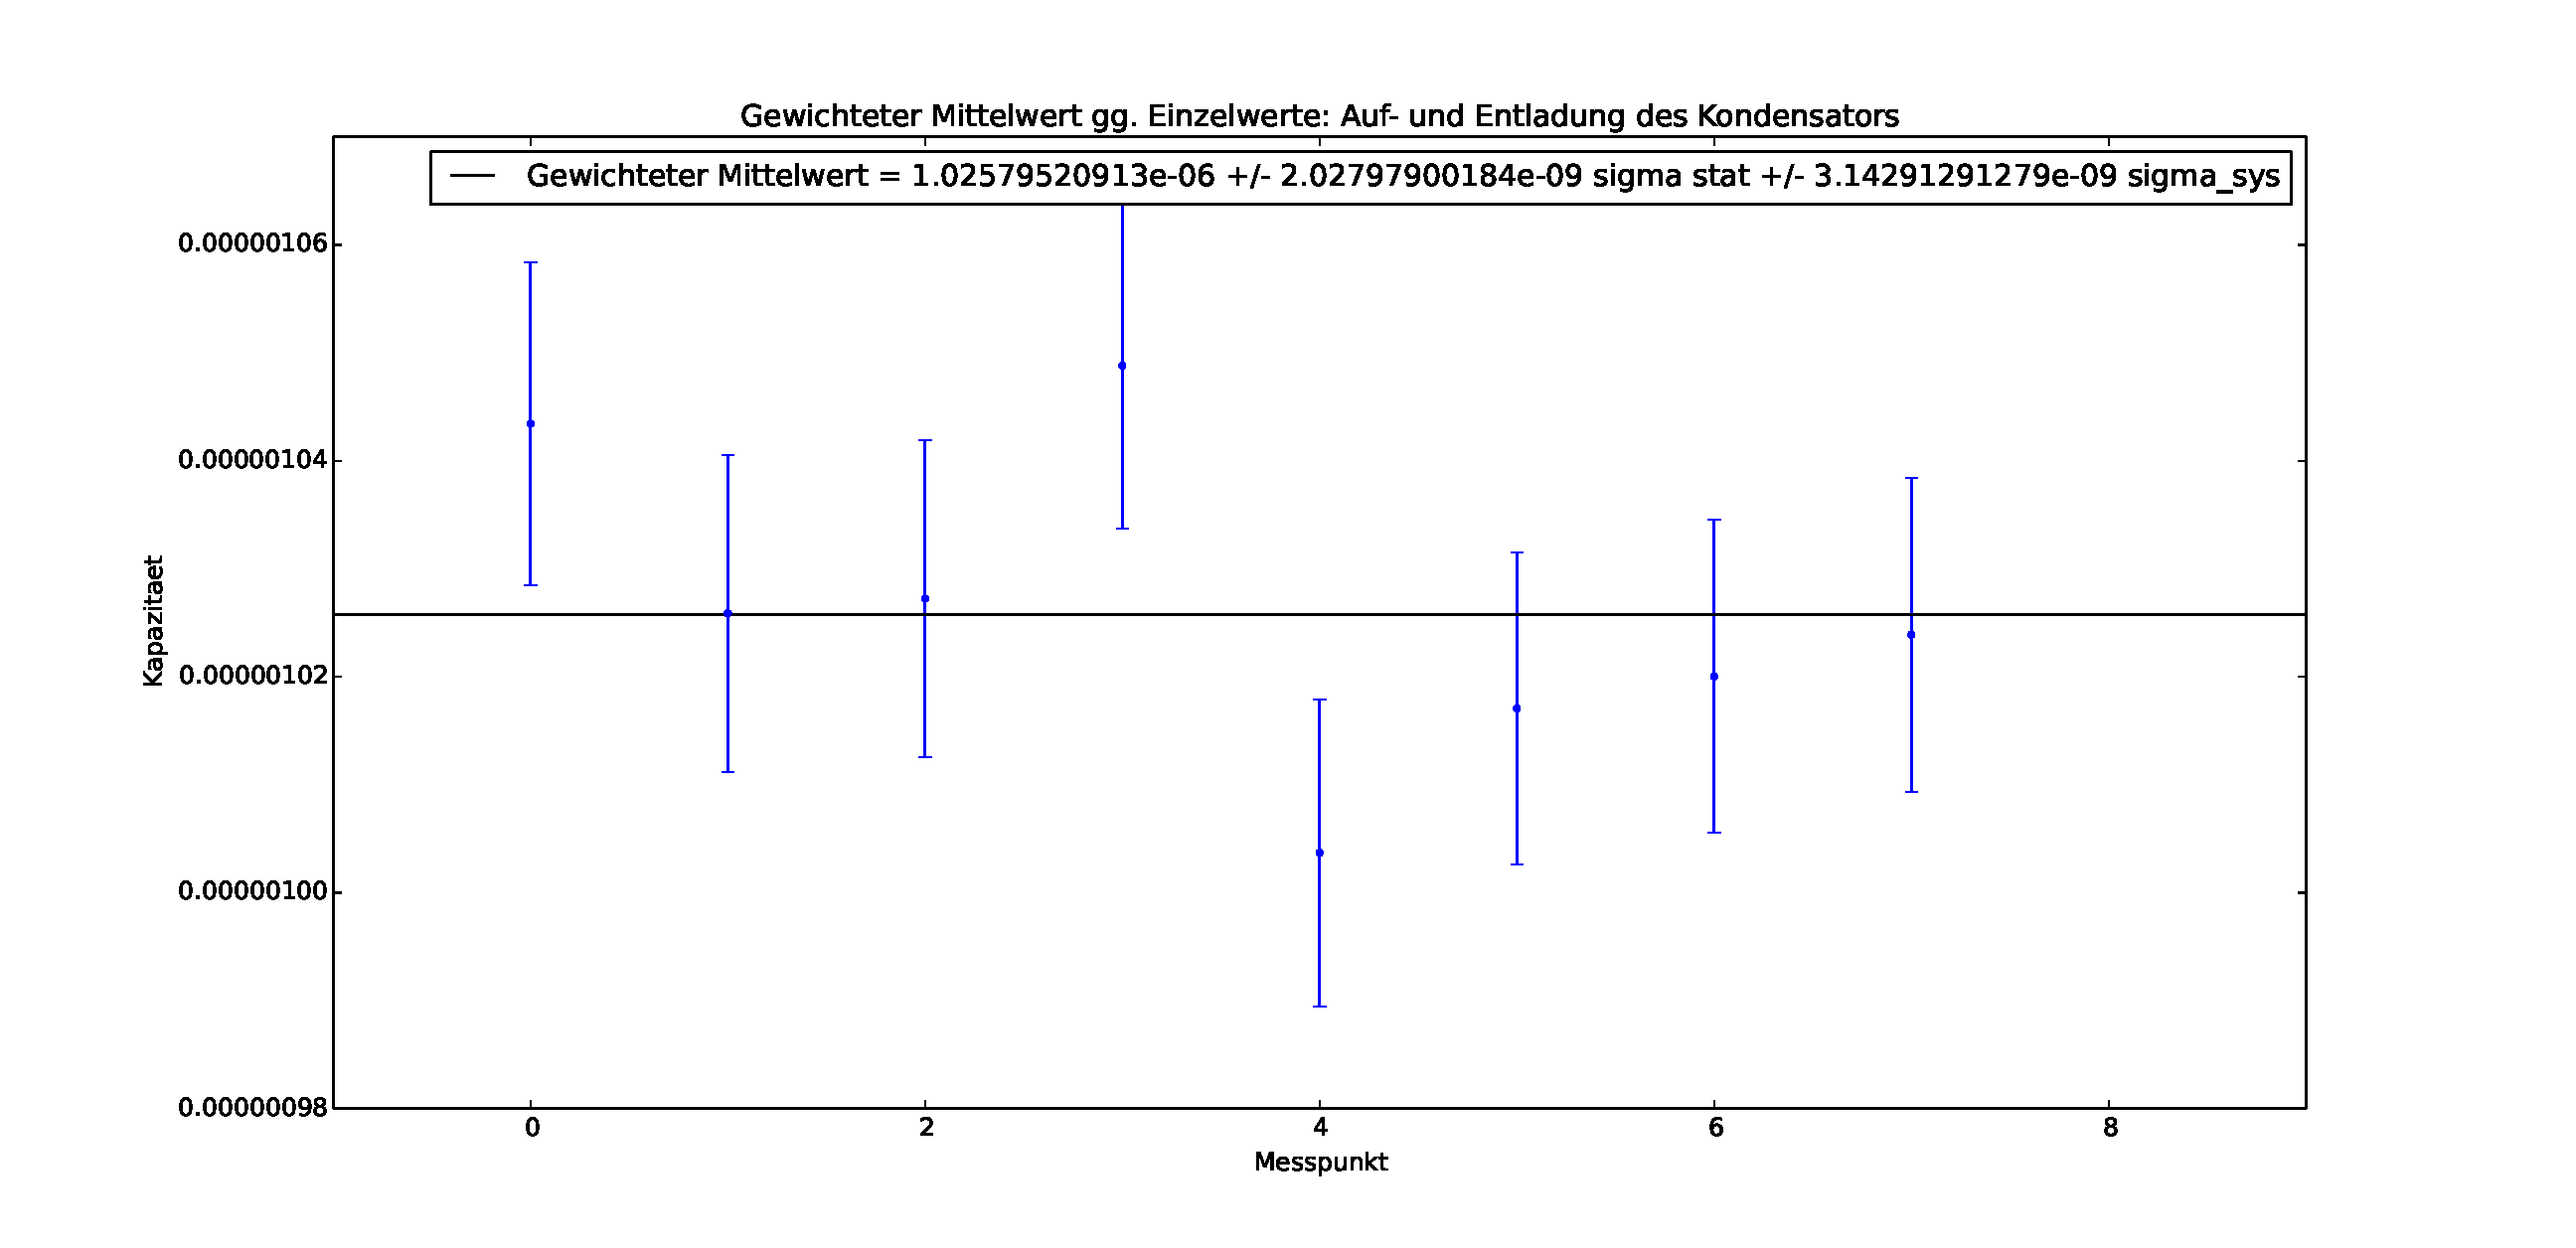
\includegraphics[scale=0.4]{verteilung_mean.eps}\\
\\Die Streuung der Einzelwerte um den gewichteten Mittelwert liegt mit ca 60\% im Rahmen der Unsicherheit auf die Einzelmessungen. Wir sind mit diesem Ergebnis sehr zufrieden.\\
\\Wir erhalten für unseren Kondensator einen Wert von: C = 1.026$\mu F \pm$ 2.028$\cdot 10^{-3}\mu F \pm$3.143$\cdot 10^{-3}\mu F$. 

\subsubsection{Fazit}
Unser Wert für C liegt mit 1.026 $\mu F$ innerhalb der 5\% Toleranzgrenze des Herstellers (0.95$\mu F$-1.05$\mu F$), unser $\chi^2$ liegt in einem zufriedenstellenden Bereich und der Wert stimmt auch mit der Vermessung des Kondensators mit der Greenbox überein (0.999$\mu F \pm$0,25\%).\\

\section{Gedämpfter LC Schwingkreis Oszilloskop, Teilversuch 4.4.1}
\subsection{Versuchsbeschreibung}
In diesem Versuch soll die Frequenz $f$ und der Dämpfungskoeffizient $\delta$ eines LRC-Schwingkreises mit Hilfe eines Oszilloskops bestimmt werden. \newline
Dazu wird die Spannung über dem Kondensator mit dem Oszilloskop aufgezeichnet, um die Frequenz und den Abklingkoeffizienten folgendermaßen zu bestimmen:
\begin{equation}
f=\frac{1}{t_{n+1}-t_n}=\frac{1}{\Delta t}
\end{equation}
\begin{equation}
\delta_n=\frac{\ln{(\frac{U_n}{U_{n+1}})}}{t_{n+1}-t_n}.
\end{equation}


\subsection{Versuchsaufbau und Durchführung}

\begin{figure}[H]
\centering
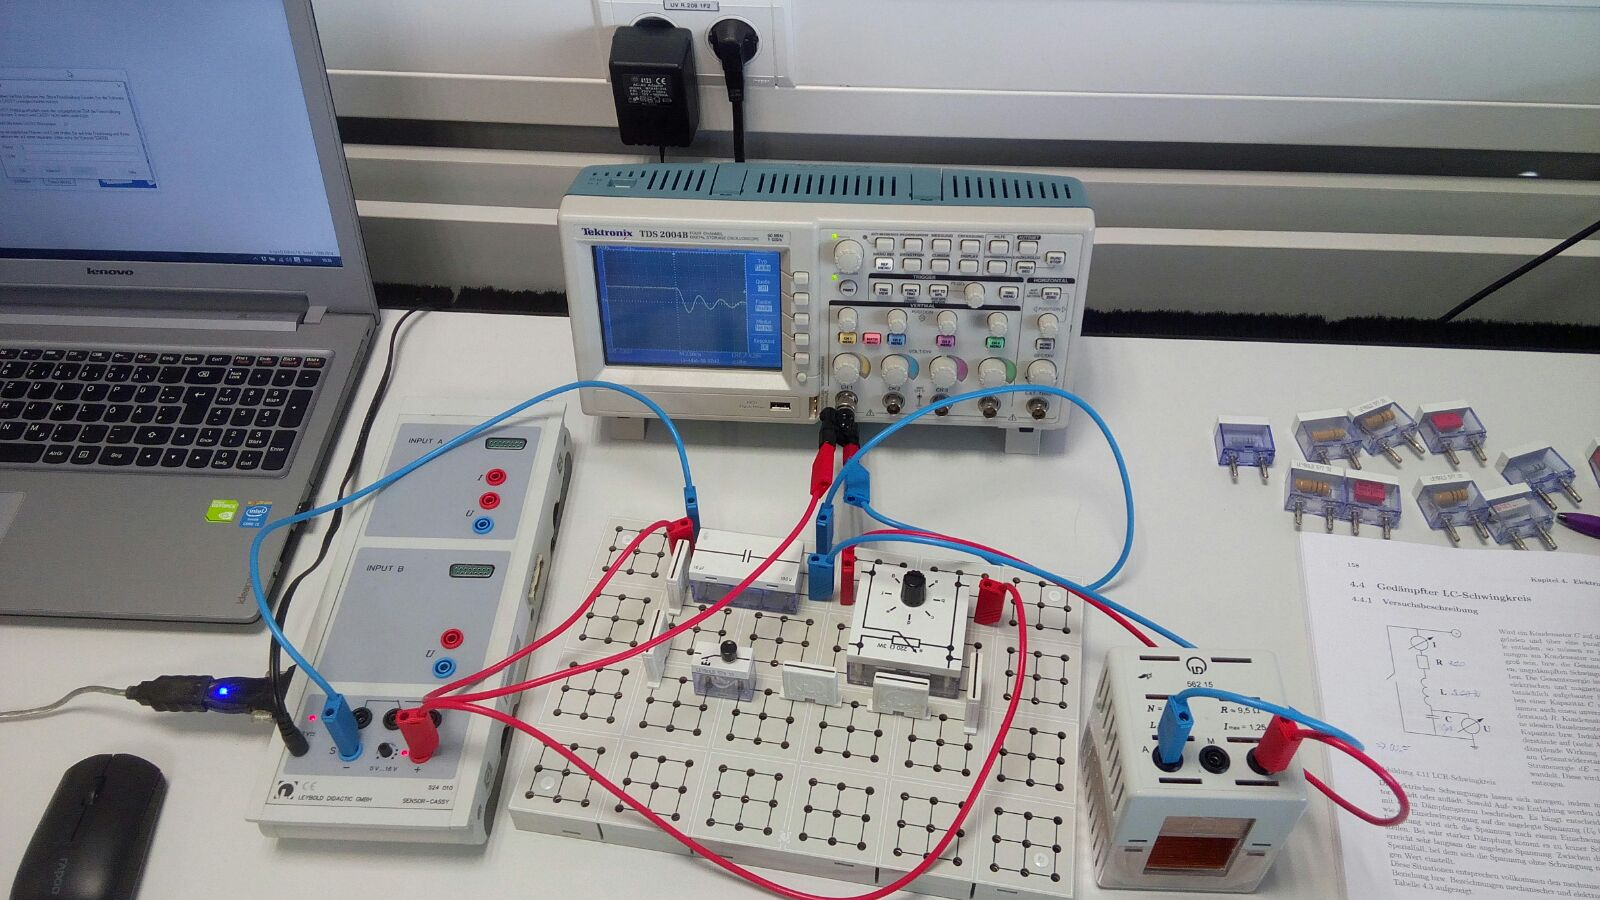
\includegraphics[scale=0.27]{ArbeitsplatzE_1.jpg}
\caption{Versuchsaufbau}
\end{figure}


\begin{itemize}
\item Bei dem oben gezeigten LRC Schwingkreis wurde der Drehwiderstand komplett herunter geregelt ($R=0.02\Omega$). Dieser wird erst später in Versuch 4.4.2 gebraucht.
 
\item Alle Versuche wurden bei einer Eingangspannung von $U_0=5.6V$ durchgeführt, dabei wurde das Oszilloskop auf \glqq Single Sequence\grqq $\,$ eingestellt und aus dem resultierenden Standbild die Spannungsmaxima mit entsprechenden Zeitwerten abgelesen. Dazu wurden die Messbereiche auf $U_B=16V$ (Spannung) \& $T_B=50 \cdot 10^{-3}s$ (Zeit) eingestellt.
\item Es lag ein Offset von $off=50 \cdot 10^{-3}V$ vor, der im Folgenden ausgeglichen wurde.
\item Die Ablesefehler wurden zu $\sigma_U=\frac{0.08}{\sqrt{12}}V$ \& $\sigma_T=\frac{100\cdot 10^{-6}}{\sqrt{12}}s$ bestimmt.
Diese Messung wurde 4 mal wiederholt wobei die Ergebnisse des 2. Versuchs aufgrund eines Stromausfalls verloren gingen.
\end{itemize}

\newpage
\subsection{Versuchsauswertung}

\subsubsection{Rohdaten}

Spule (Herstellerangaben): 
\begin{figure}[H]\centering
\begin{tabular}{c|l}
Induktivität & $L=36*10^{-3}H$\\ 
Windungen & $N=1000$\\ 
Widerstand & $R=9.5\Omega$ \\
\end{tabular} 
\end{figure}

Kondensator (Herstellerangabe):
\begin{figure}[H]\centering
\begin{tabular}{c|l}
Kapazität & $C=10*10^{-6}F$\\ 
\end{tabular} 
\end{figure}

Messdaten:
\begin{table}[H]\centering
\caption{1. Messung}
\begin{tabular}{c|c}
\hline
$U_1=3.12V$& $t_1=0.5ms$\\ 
$U_2=1.76V$& $t_2=4.4ms$\\ 
$U_3=1.04V$& $t_3=8.2ms$ \\
$U_4=0.56V$& $t_4=12.0ms$ \\
\end{tabular} 
\end{table}

2. Messung fehlt wegen Stromausfall.

\begin{table}[H]\centering
\caption{3. Messung}
\begin{tabular}{c|c}
\hline
$U_1=3.2V$& $t_1=0.5ms$\\ 
$U_2=1.76V$& $t_2=4.4ms$\\ 
$U_3=1.04V$& $t_3=8.2ms$ \\
$U_4=0.64V$& $t_4=12.0ms$ \\
$U_5=0.4V$& $t_4=15.9ms$ \\
\end{tabular} 
\end{table}

\begin{table}[H]\centering
\caption{4. Messung}
\begin{tabular}{c|c}
\hline
$U_1=3.12V$& $t_1=0.5ms$\\ 
$U_2=1.76V$& $t_2=4.4ms$\\ 
$U_3=1.12V$& $t_3=8.2ms$ \\
$U_4=0.8V$& $t_4=12.1ms$ \\
$U_5=0.4V$& $t_4=15.9ms$ \\
\end{tabular} 
\end{table}

$U_4$ und $T_4$ wurden bei Messung4 wegen falschem Ablesen verworfen.

\begin{figure}[H]\centering
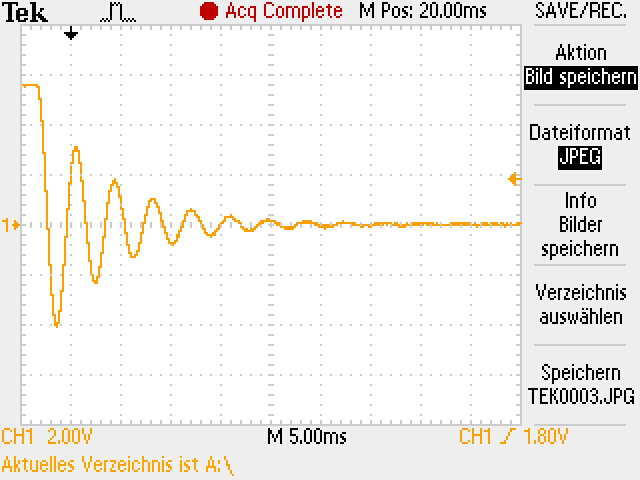
\includegraphics[scale=0.7]{TEK0003.JPG}
\caption{Beispiel: Messung 1}
\end{figure}


\newpage
\subsubsection{Transformation der Rohdaten}
Die Frequenzen wurden aus den Differenzen der Zeitabstände $T_i$ bestimmt. Bestimmung von Delta siehe Gleichung (\ref{Peter}). \\
Beispiel:

\begin{table}[H]\centering
\caption{Messung 1}
\begin{tabular}{c|c|c|c}
Frequenz in Hz & $\sigma_f$ in Hz & Abklingkoeffizient in $\frac{1}{s}$ & $\sigma_{\delta}$ in $\frac{1}{s}$\\ 
\hline
$f=256.410$& $\sigma_f=1.898$& $\delta=150.047$& $\sigma_{\delta}=4.264$\\ 
$f=263.158$& $\sigma_f=1.999$& $\delta=143.827$& $\sigma_{\delta}=7.260$\\
$f=263.158$& $\sigma_f=1.999$& $\delta=174.551$& $\sigma_{\delta}=13.535$\\
\end{tabular} 
\end{table}
Hier wurden die Fehler aus den folgenden Gleichungen ermittelt:
\begin{align}
\sigma_f&=\frac{\sigma_T}{T^2}\\
\sigma_{\delta_n}&=\frac{1}{T_n}\cdot \sqrt{(\frac{\sigma_{U_n}}{U_n})^2+(\frac{\sigma_{U_{n+1}}}{U_{n+1}})^2+(\delta_n\cdot \sigma_{T_n})^2}
\end{align}
Der Abklingkoeffizient $\delta$ wird bestimmt aus:

\begin{align}
U_{n+1}&=U_n \cdot e^{-\delta \cdot (t_{n+1}-t_n)}\notag \\
\Rightarrow \hspace{0.5cm} \delta_n&=\frac{\ln{\frac{U_n}{U_{n+1}}}}{t_{n+1}-t_n}
\label{Peter}
\end{align}
\newline
Aus den Einzelmessungen haben wir für die Frequenz und den Abklingkoeffizient den gewichteten Mittelwert mit seinem Fehler bestimmt:

\begin{table}[H]\centering
\caption{Ergebnis}
\begin{tabular}{c|c|c|c|c|c}
$\bar{f}$ in Hz & $\sigma_{\bar{f}}$ in Hz & $f_{Theo}$ & $\bar{\delta}$ in $\frac{1}{s}$ & $\sigma_{\bar{\delta}}$ in $\frac{1}{s}$& $\delta_{Theo}$ \\ 
\hline
$259.960$& $0.617$ & $264.426$ & $148.025$& $1.994$& $131.944$\\ 
\end{tabular} 
\end{table}

\begin{figure}[H]
\caption{Frequenz}
\centering
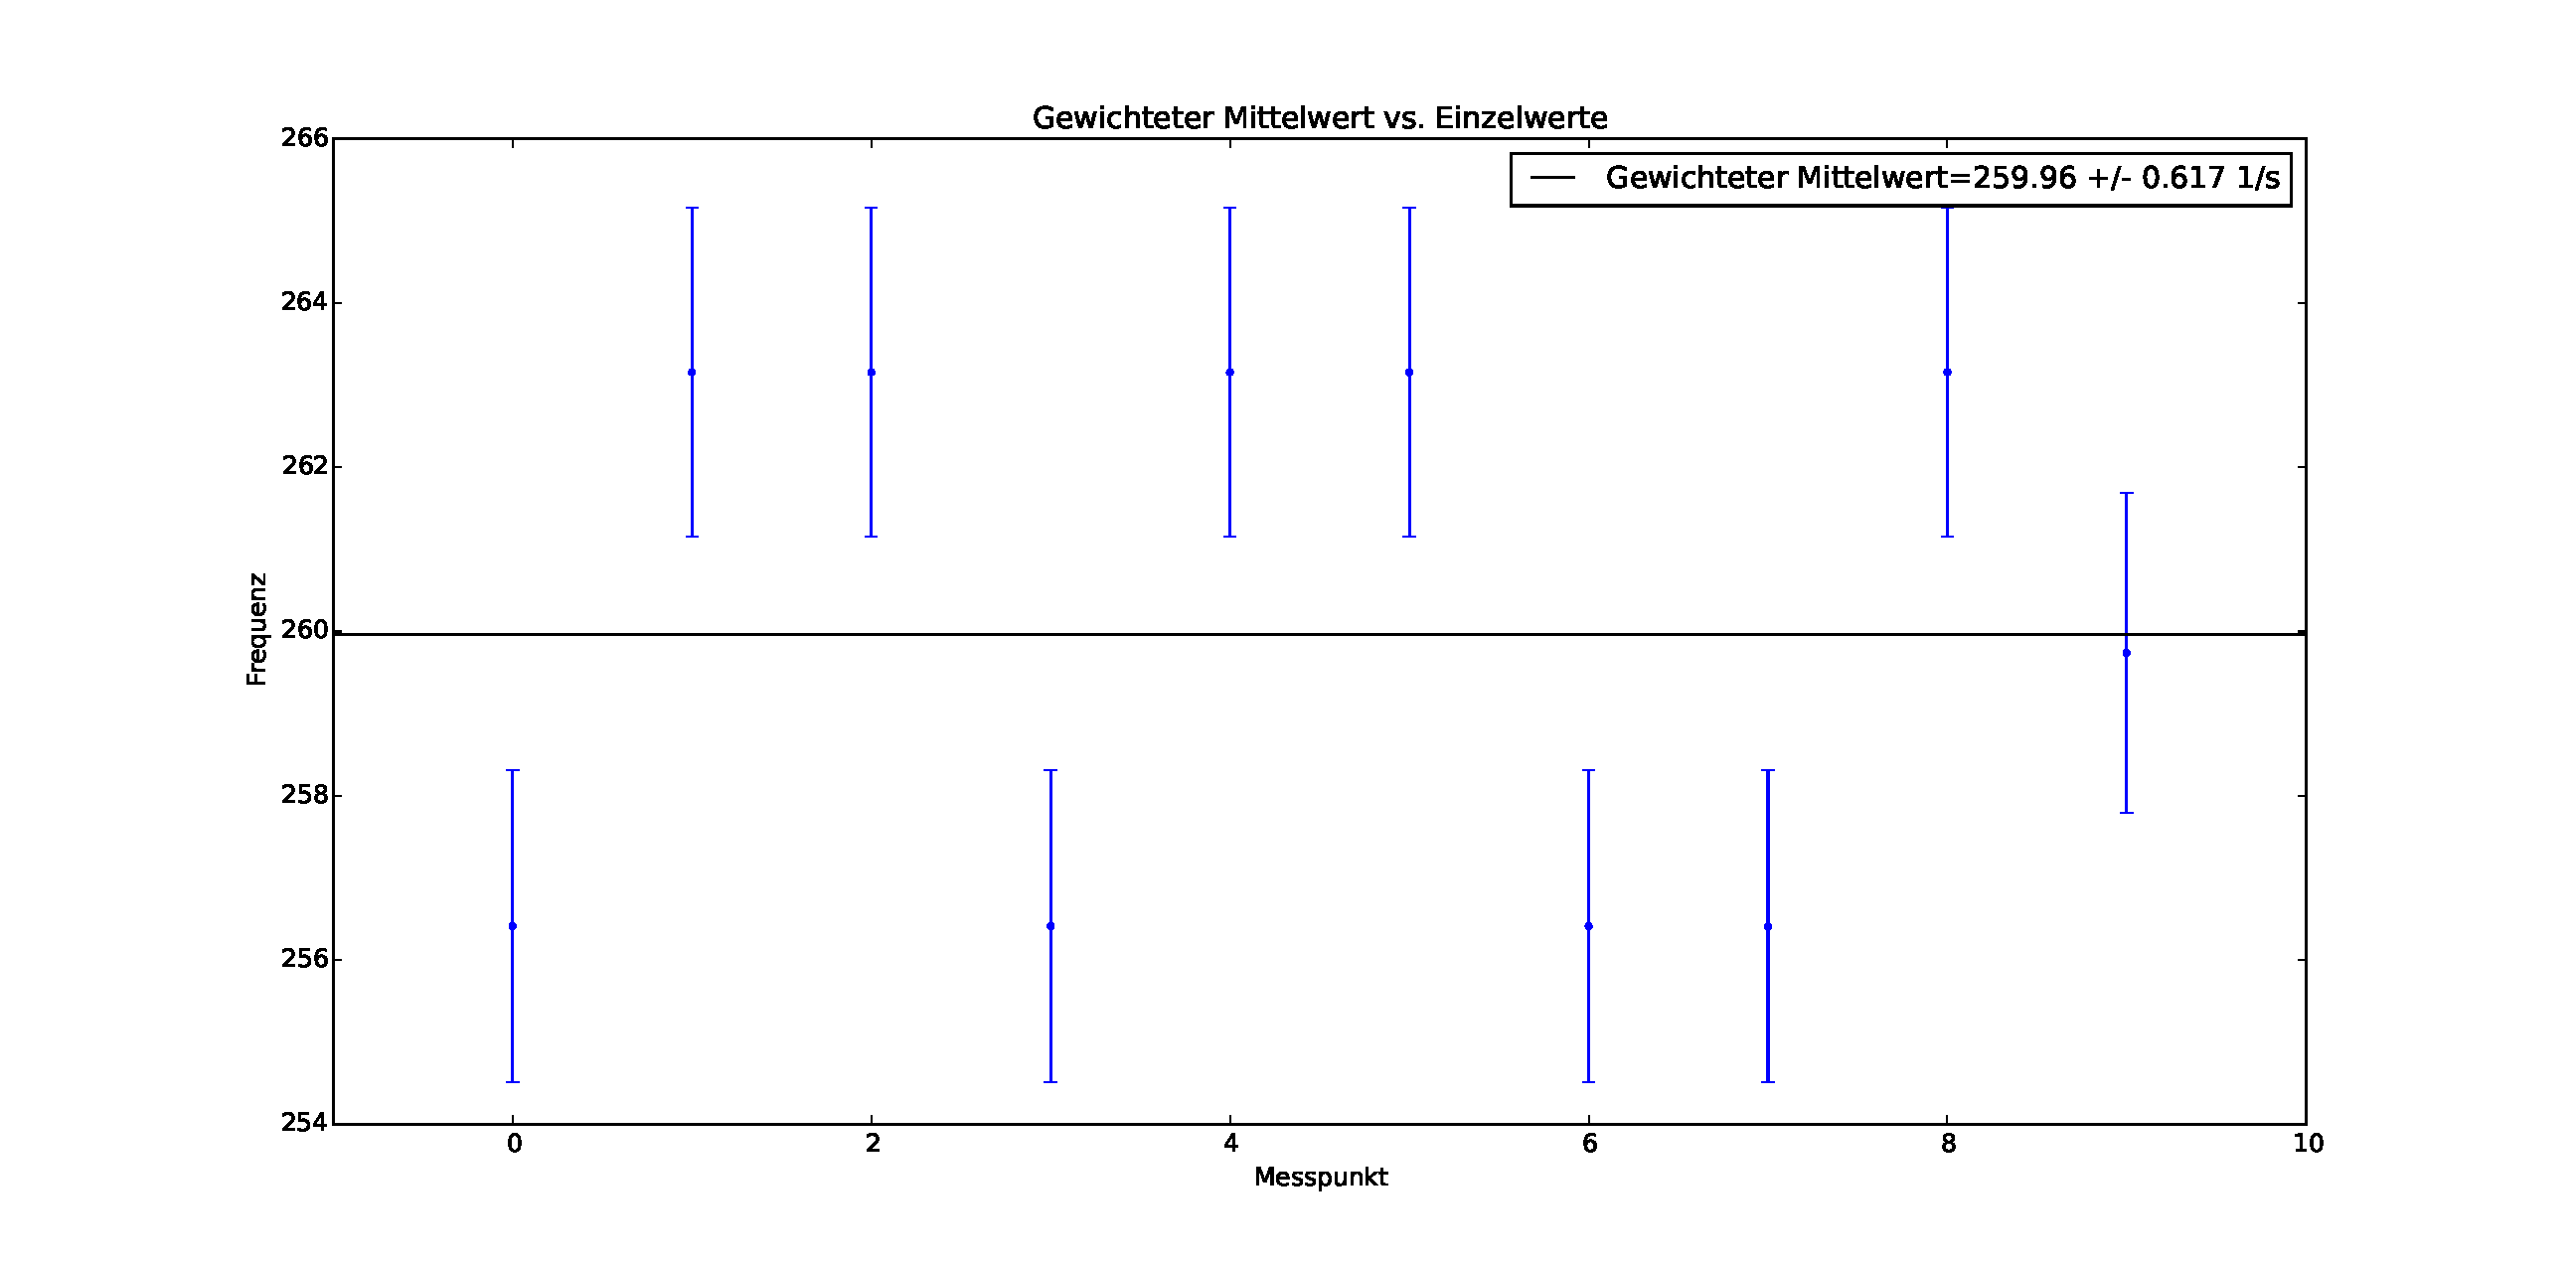
\includegraphics[scale=0.3]{Bilder/FrequenzGewichtet.eps}
\label{Frequenz_Oszi}
\end{figure}

\begin{figure}[H]
\caption{Abklingkoeffizient}
\centering
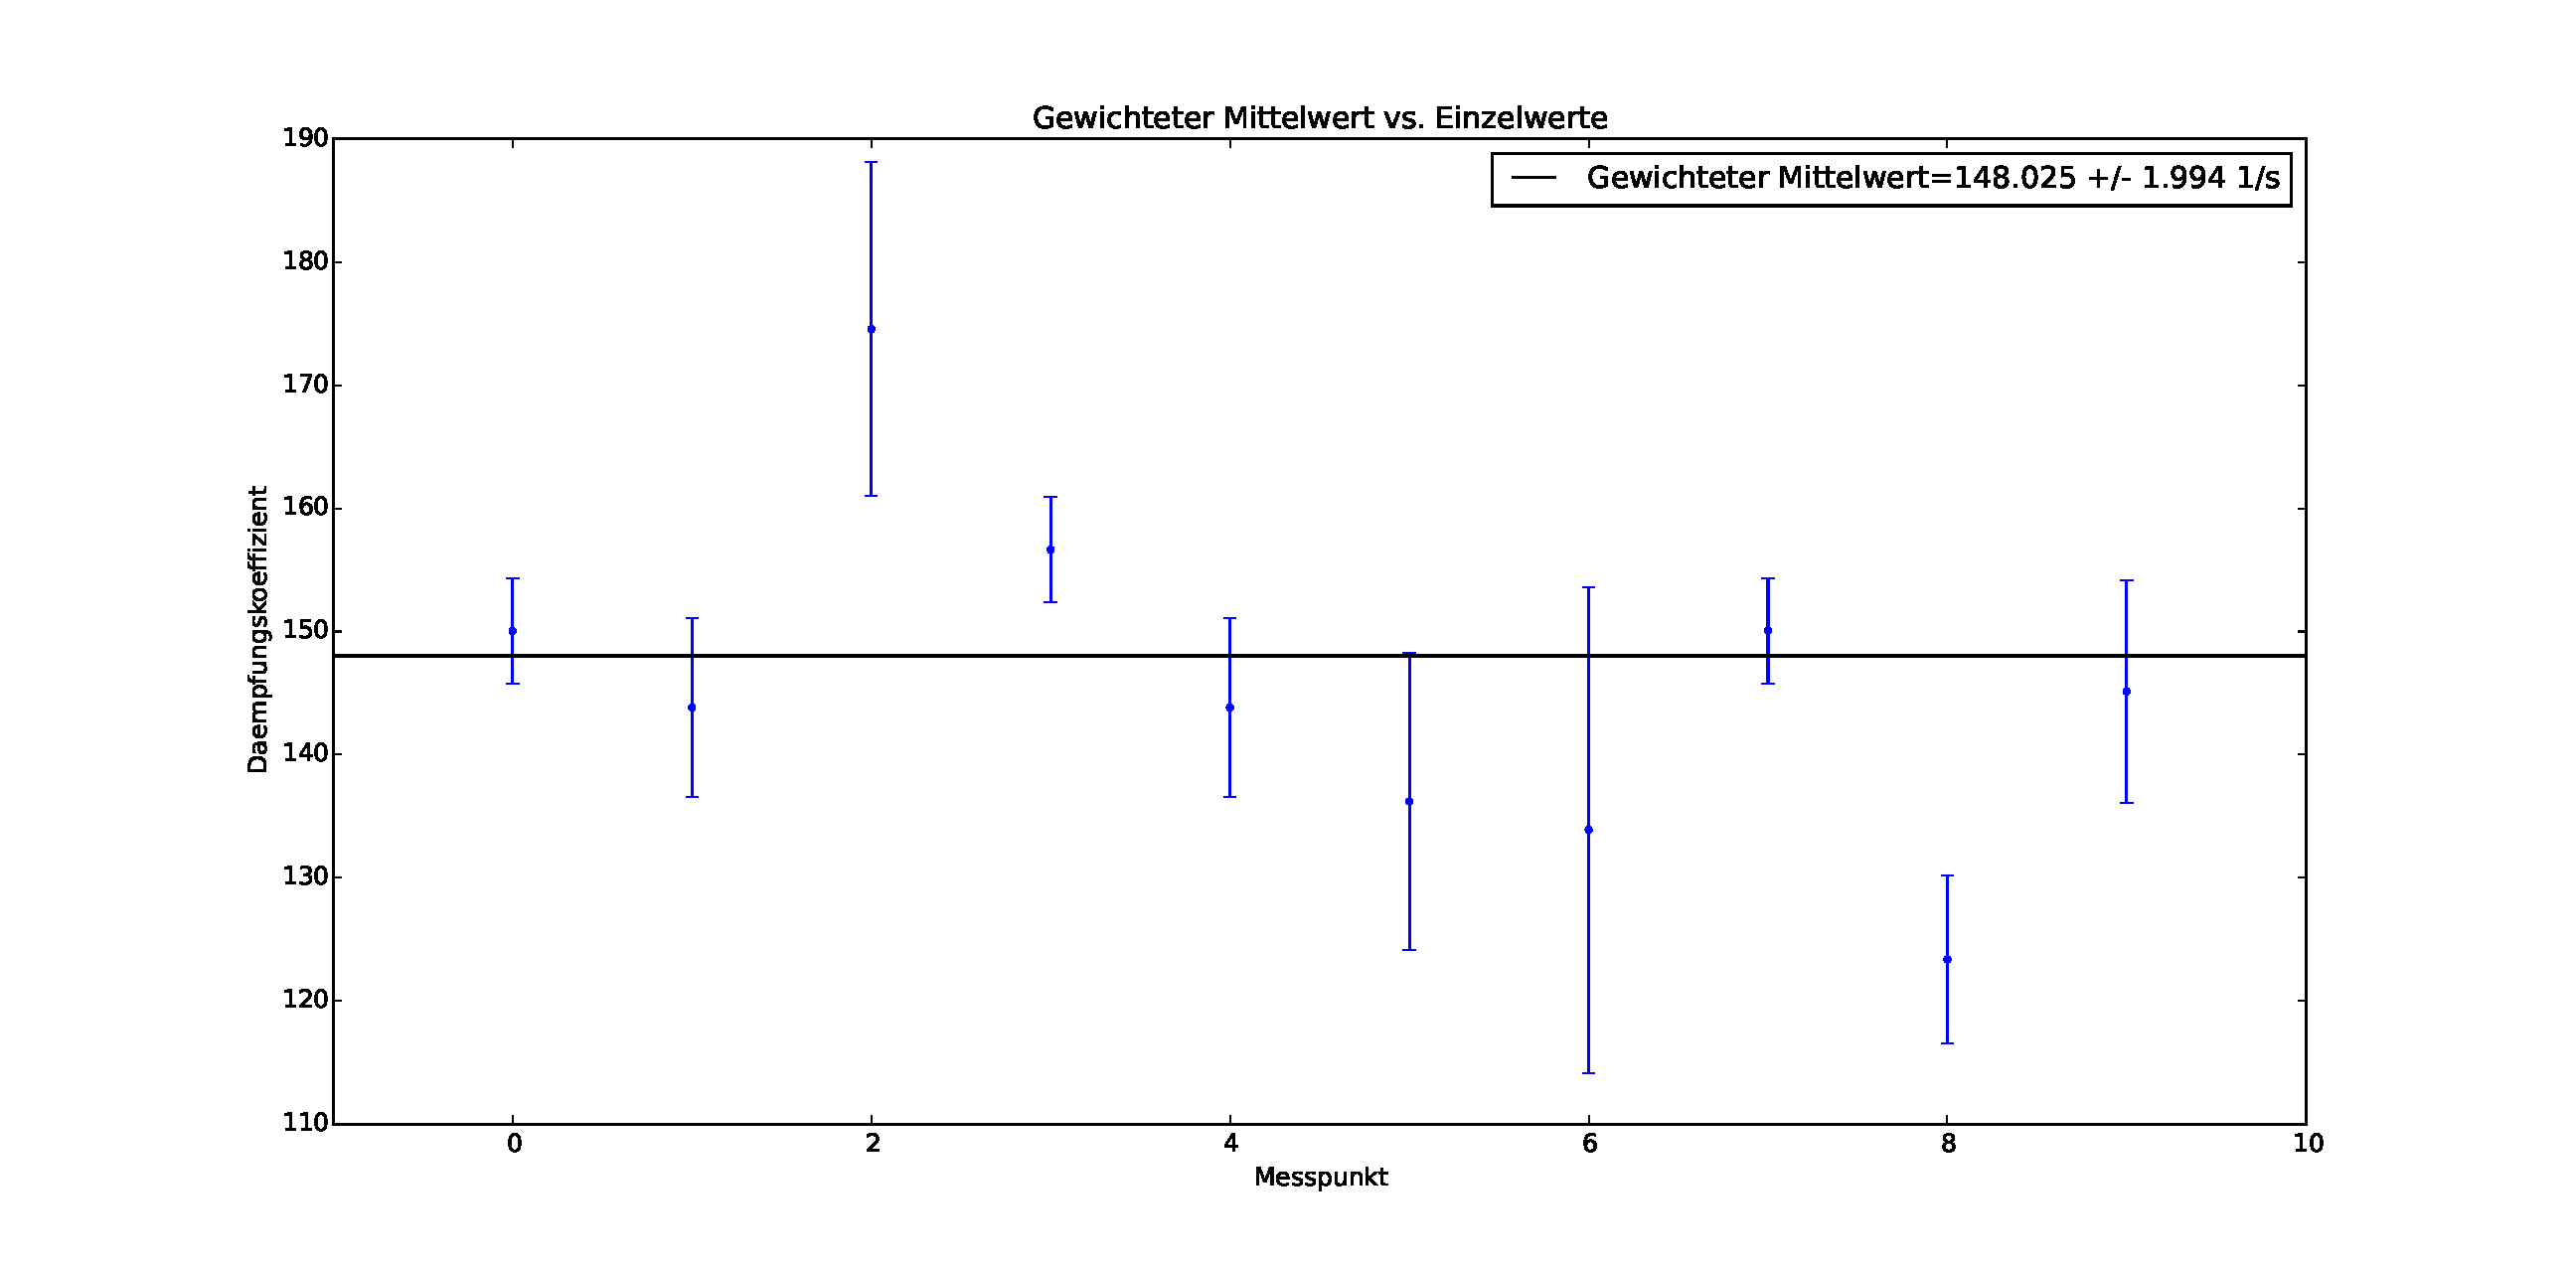
\includegraphics[scale=0.3]{Bilder/DaempfungGewichtet.eps}
\end{figure}


\subsubsection{Analyse und Fazit}
Auffällig ist, dass die gemessene Frequenz kleiner ist, als die theoretische Frequenz. Da die theoretische Frequenz allerdings allein aus den Herstellerangaben berechnet wurde ist ein ähnlicher Wert kaum zu erwarten. 
\newline
Weiterhin fällt auf, dass $\delta$ größer ist als $\delta_{theo}$. Der Grund dafür ist, dass $\delta \sim R$ und wir bei R mit Sicherheit einen höheren Wert erwarten müssten, da zum Beispiel alle Bauteile einen Innenwiderstand aufweisen. 
\newline
Die jeweiligen Fehler auf die Mittelwerte liegen in einem realistischen Rahmen.
\newline
Abbildung \ref{Frequenz_Oszi} zeigt einen zugegebenermaßen seltsamen Verlauf. Vier der Werte liegen auf extrem gleicher Höhe unter dem Graphen, fünf Werte auf ebenso gleicher Höhe über dem Graphen. Nur ein Fehlerbalken schneidet den Mittelwert. Wir erklären uns dies dadurch,  dass die gemessenen Zeitpunkte und deren Differenzen im Rahmen der Auflösung am Oszilloskop immer gleich waren (siehe Zeitmessung in Rohdaten).   
\newline
Erweitert man den Fehler auf $2\cdot\sigma$ ergibt sich, dass alle Fehler den Mittelwert schneiden.  
\begin{figure}[H]
\caption{Frequenz 2$\sigma$ }
\centering
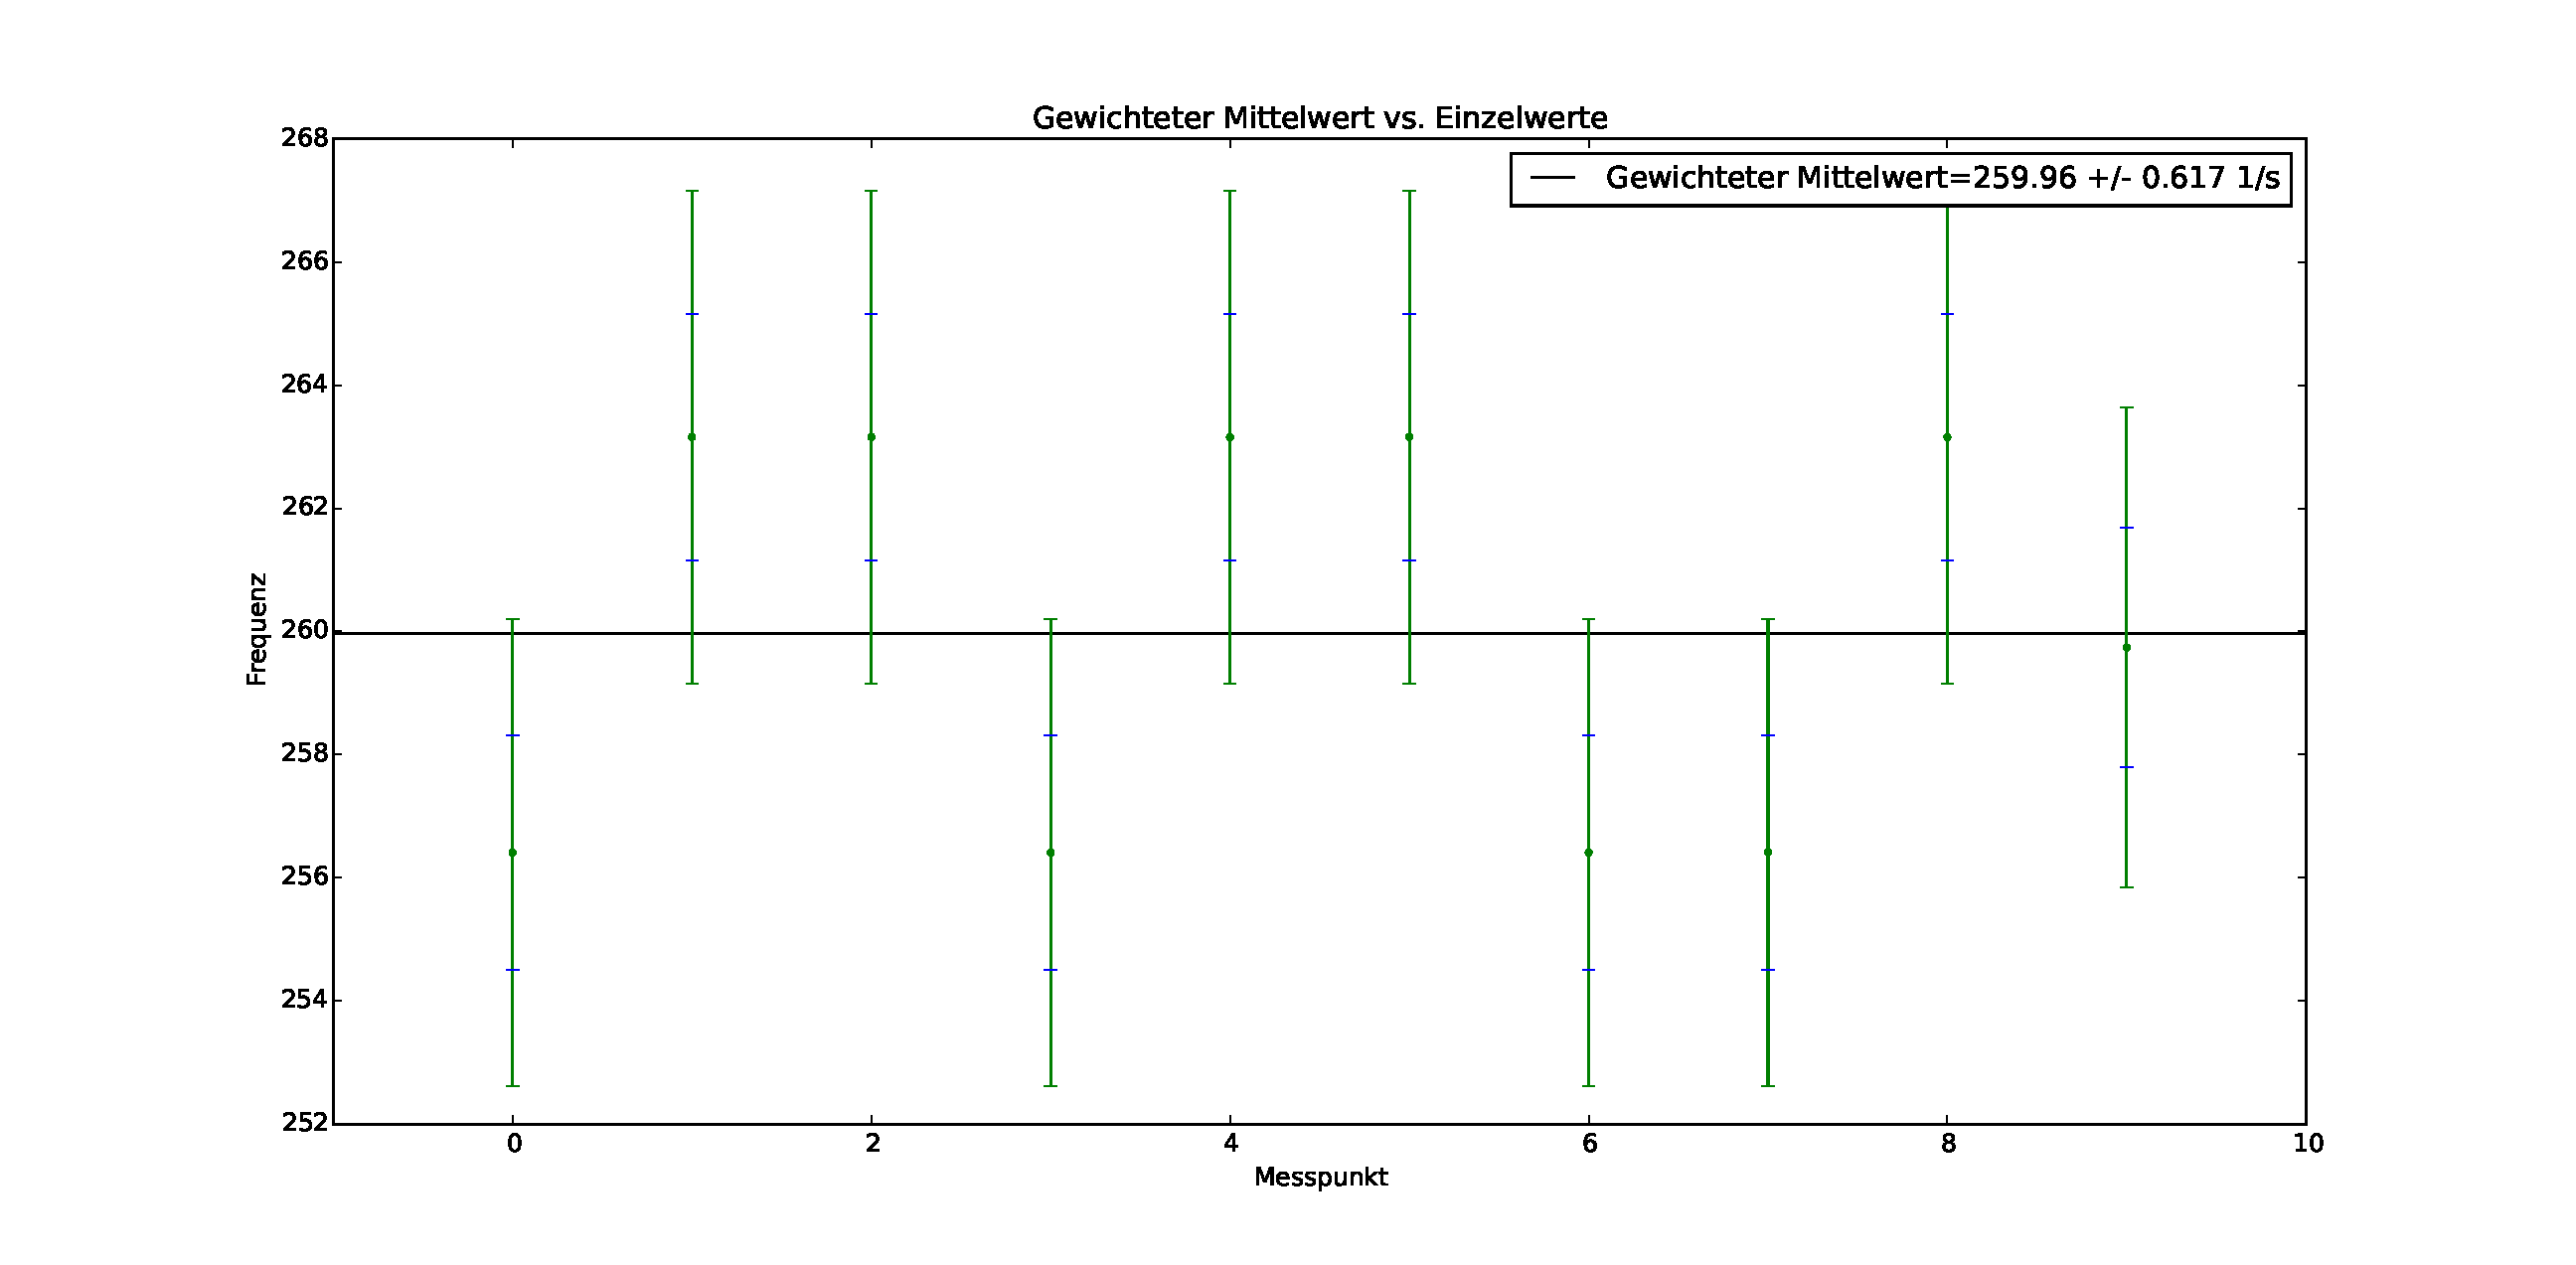
\includegraphics[scale=0.35]{Bilder/FrequenzGewichtetZweiSigma.eps}
\end{figure}

Der Plot zum Abklingkoeffizient sieht sehr vernünftig aus. Zwar schneiden nur 7 von 10 Fehlerbalken den Mittelwert, dies ist aber zu erwarten, da theoretisch nur $\approx 68\%$ der Werte den Mittelwert schneiden sollten.

\section{Gedämpfter LC Schwingkreis Cassy, Teilversuch 4.4.2}
\subsection{Versuchsbeschreibung}

Beim Teilversuch 4.4.2 sollte zunächst die Messung der Frequenz $f$ und die Messung des Dämpfungskoeffizienten $\delta$ wie in Teilversuch 4.4.1 wiederholt werden, nur dieses Mal sollte die Messung über das Sensor-Cassy statt über das Oszilloskop erfolgen.
Die Frequenz und der Dämpfungskoeffizient berechnen sich dabei nach den gleichen Formeln wie zuvor.
Die Schaltung sollte durch einen variierbaren Widerstand erweitert werden und mindestens ein Kriechfall($D=\frac{\delta}{\omega}>1$), ein Schwingfall($D<1$) und ein aperiodischer Grenzfall($D=1$) aufgenommen werden.
\newline
Nachdem die Dämpfungskonstante $\delta$ bestimmt wurde, konnte daraus die Induktivität der Spule über:
\begin{equation}
\delta =\frac{R}{2L} \hspace{1cm}
\Leftrightarrow  \hspace{1cm} L=\frac{1}{2\delta}\cdot R \label{Spule}
\end{equation}
bestimmt werden.
\newline
Für den aperiodischen Grenzfall gilt:
\begin{equation}
R_{ap}=2\cdot\sqrt{\frac{L}{C}}.
\label{aperiodischer GF}
\end{equation}
Dieser Grenzfall sollte mit Hilfe des Drehwiderstandes eingestellt und mit der Vorhersage verglichen werden.
\subsection{Versuchsaufbau}

Der Versuch wurde wie in der folgenden Skizze aufgebaut.

\begin{figure}[H]
    \subfigure[Versuchsaufbau aus dem Skript]{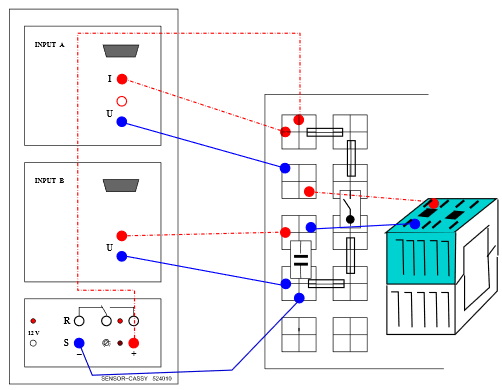
\includegraphics[width=0.49\textwidth]{Bilder/VersuchsaufbauOhneWiderstand.PNG}}
    \subfigure[unser Versuchsaufbau mit Widerstand]{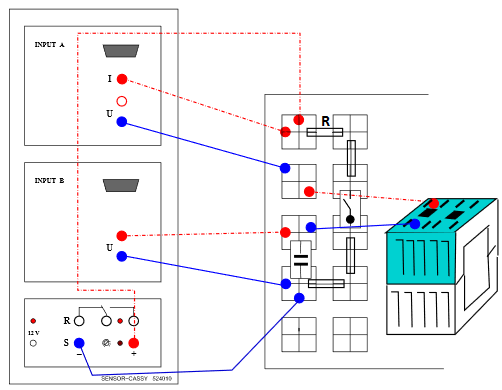
\includegraphics[width=0.49\textwidth]{Bilder/VersuchsaufbauMitWiderstand.PNG}}
\caption{Versuchsaufbau}
\end{figure}

Dabei wurde die Schaltung aus Teilversuch 4.4.1 fast gänzlich übernommen. Lediglich wurde das Oszilloskop durch ein Sensor Cassy ersetzt. Die Werte für die Spule, den Kondensator und die Eingangsspannung entsprechen daher denen aus Teilversuch 4.4.1.
Der skizzierte Dreh-Widerstand wurde auch im Aufbau zuvor benutzt allerdings auf null ($\approx$ 0.02 $\Omega$) gedreht.
\newline
Die Messbereiche wurden folgendermaßen eingestellt:
\begin{equation}
U_B=\pm 10 V \hspace{1cm} T_B=40 ms.
\end{equation}
Da wir die Schwingung eines sich entladenden gedämpften LRC-Schwingkreises bei einer Eingangsspannung von etwa $5.62V$ gemessen haben, haben wir den Trigger der Spannungsmessung auf ab $5.5V$ fallend eingestellt.
\newline

\subsection{Durchführung}
Insgesamt haben wir 34 Einzelmessungen durchgeführt. 
Dabei haben wir für die Messung der Induktivität unterschiedliche Widerstände über den Drehwiderstand eingestellt und gemessen. Für die Messung der Frequenz und des Dämpfungskoeffizienten haben wir mehrere Schwingungen für den selben Widerstand gemessen. Bei weiteren Messungen haben wir die Messzeit extrem verlängert, um einen eventuellen Offset besser abzuschätzen.
\newline
\newline
Für die Aufzeichnung eines Kriechfalls haben wir den Drehwiderstand durch einen $1k\Omega$ Widerstand ersetzt. Damit konnte sichergestellt werden, dass $D\gg 1$ und somit ein Kriechfall vorliegt.
\newline
Für die Aufzeichnung des aperiodischen Grenzfalls haben wir zunächst den nötigen Widerstand über Gleichung \ref{aperiodischer GF} abgeschätzt. Bei den gegeben Werten für R und L gilt dann:
\begin{equation}
R_{ap}\approx 120\Omega.
\end{equation}
Der Drehwiderstand musste also in diesen Bereich eingestellt und beobachtet werden ob bei der Schwingung die entsprechende Charakteristik vorliegt.
\newline
Für die Messung von $f,\delta$ und $L$ wurden Schwingfälle benötigt. Daher wurden hier Widerstände eingestellt, die deutlich unter $R= 120\Omega$ liegen.

\begin{figure}[H]
\caption{Aufbau}
\centering
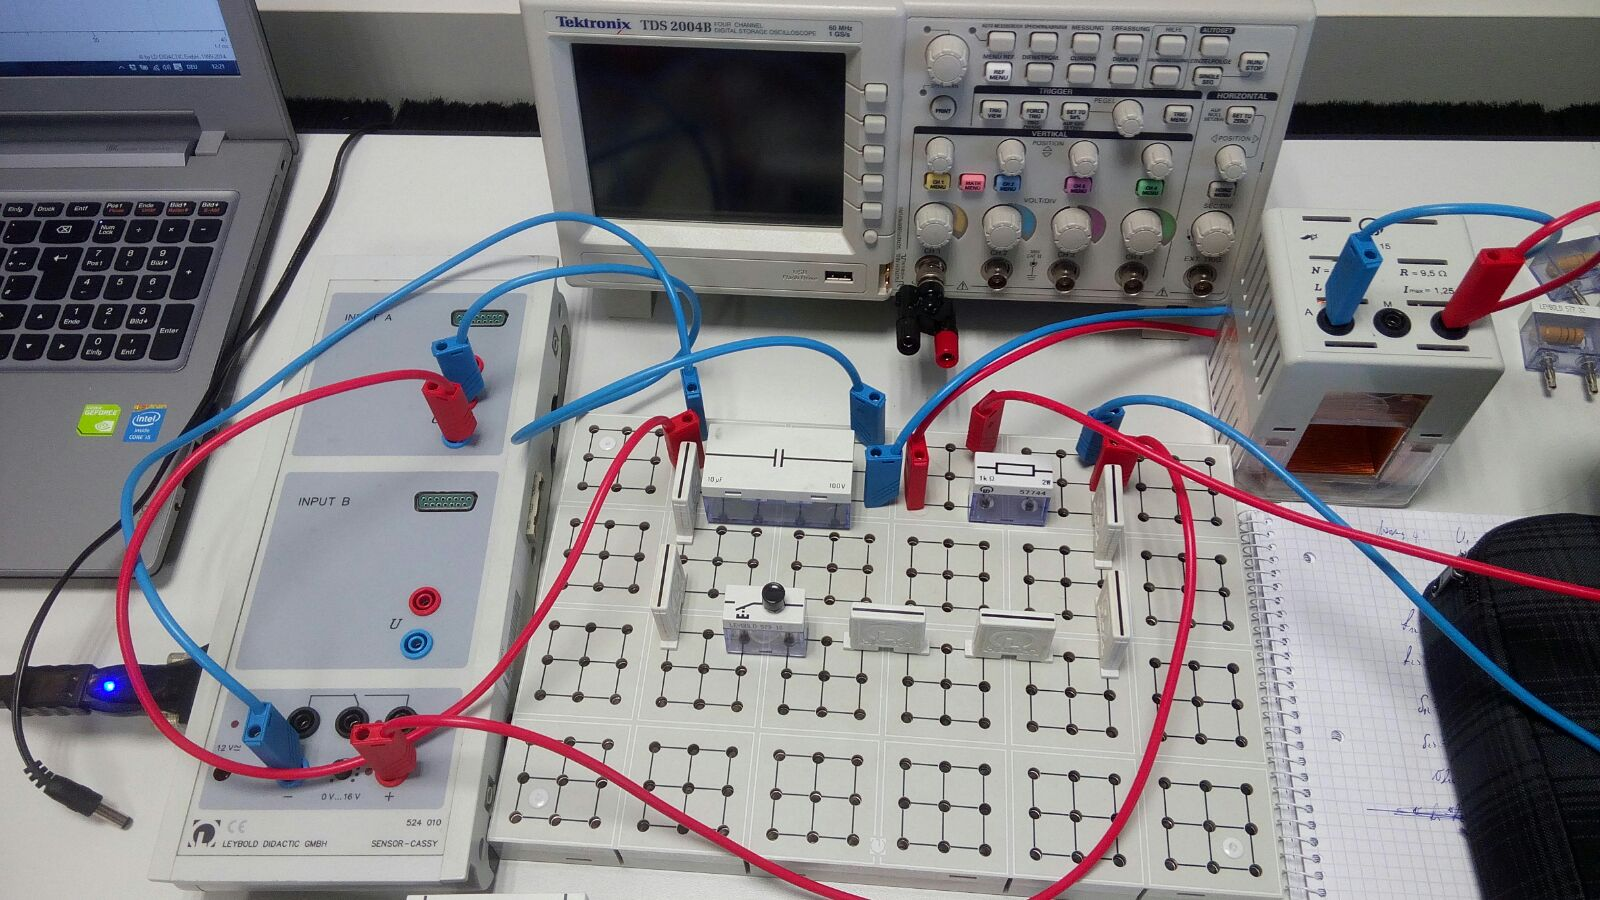
\includegraphics[scale=0.25]{Bilder/AufbauFoto.jpg}
\end{figure}



\newpage
\subsection{Versuchsauswertung}

\subsubsection{Rohdaten}
Bei der Vermessung mit dem Cassy wurde dieselbe Spule, derselbe Kondensator und dieselbe Eingangsspannung wie in Teilversuch 4.4.1 verwendet.

Aus der Auflösung des Cassy folgen Ablesefehler von:
\begin{equation}
\sigma_U=\frac{0.01V}{\sqrt{12}} \hspace{1cm}
\sigma_T=\frac{0.03ms}{\sqrt{12}}
\end{equation}

Im Folgenden sind Beispielmessungen abgebildet.

\begin{figure}[H]
\caption{Schwingfall bei $R\approx 0.02\Omega$ mit Bestimmung des Offsets}
\centering
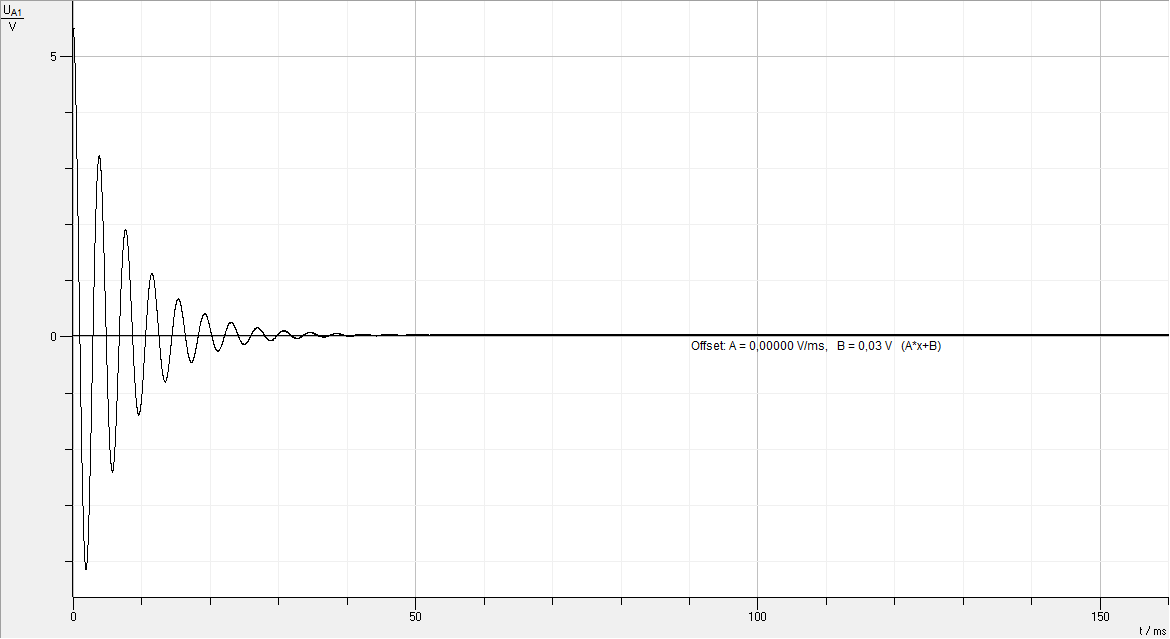
\includegraphics[scale=0.3]{Bilder/SchwingfallMitOffset0Ohm.png}
\end{figure}

\begin{figure}[H]
\caption{Schwingfall bei $2.4\Omega$}
\centering
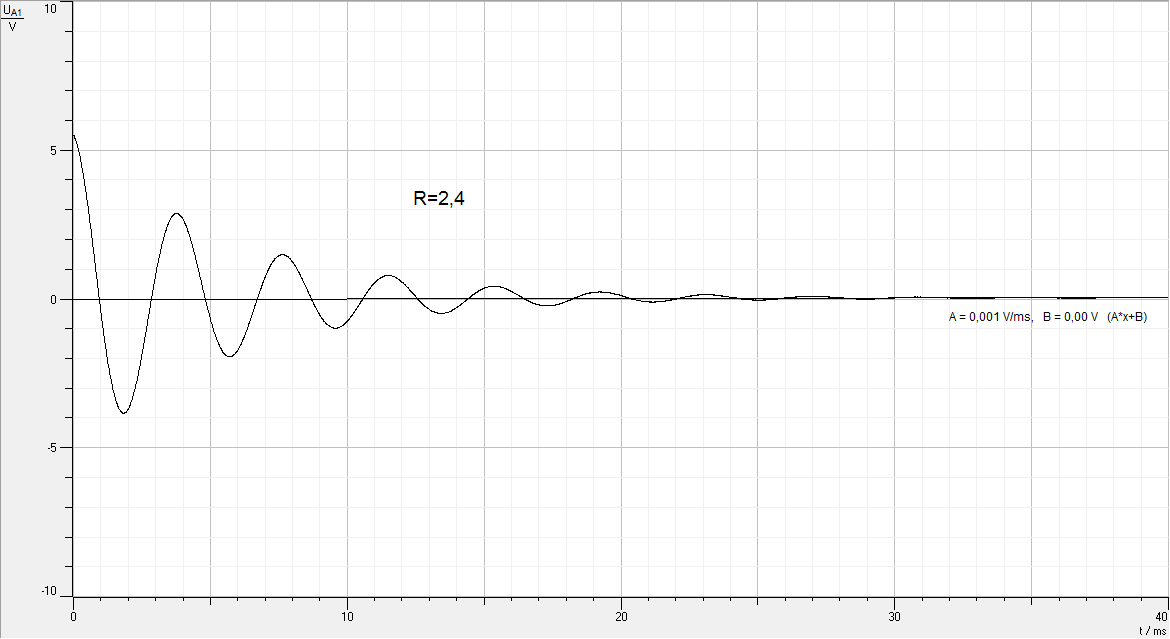
\includegraphics[scale=0.3]{Bilder/Schwingfall2komma4Ohm.png}
\end{figure}


\begin{figure}[H]
\caption{Kriechfall bei R=1k$\Omega$}
\centering
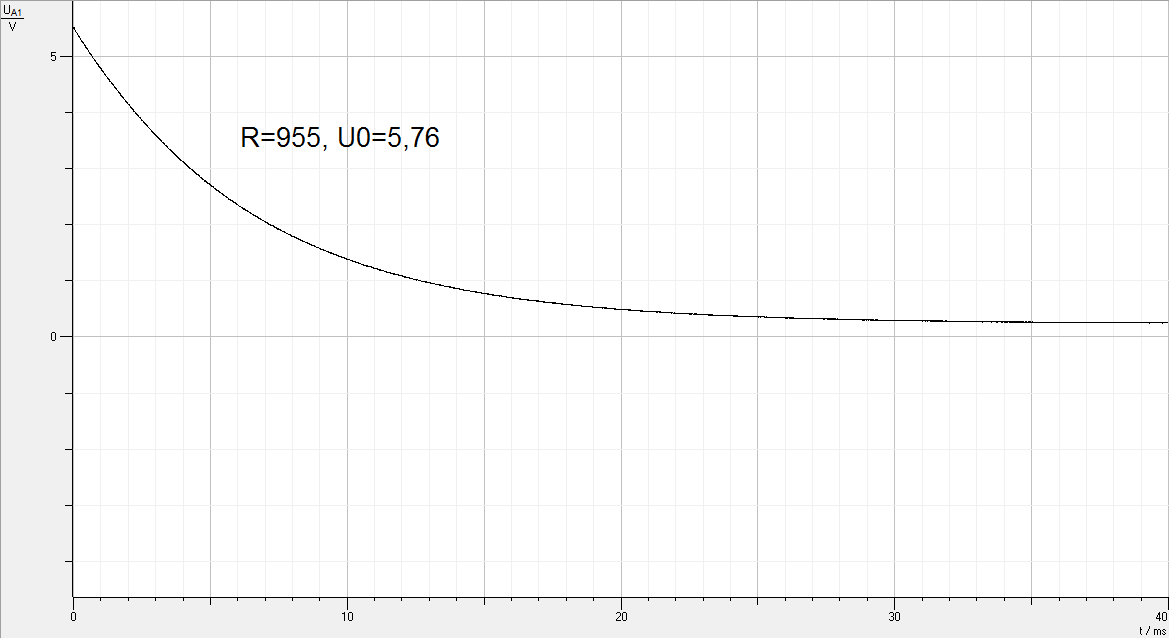
\includegraphics[scale=0.3]{Bilder/Kriechfall1KOhm.png}
\end{figure}




\subsubsection{Transformation der Rohdaten}
\textbf{Bestimmung der Frequenz durch FFT}: \\
Mithilfe der in Cassy eingebauten Fast-Fourier-Transformation(FFT) lässt sich sehr schnell die Frequenz einer Schwingung bestimmen:

\begin{figure}[H]
\caption{Bestimmung der Frequenz bei $R=2.4\Omega$ durch FFT}
\centering
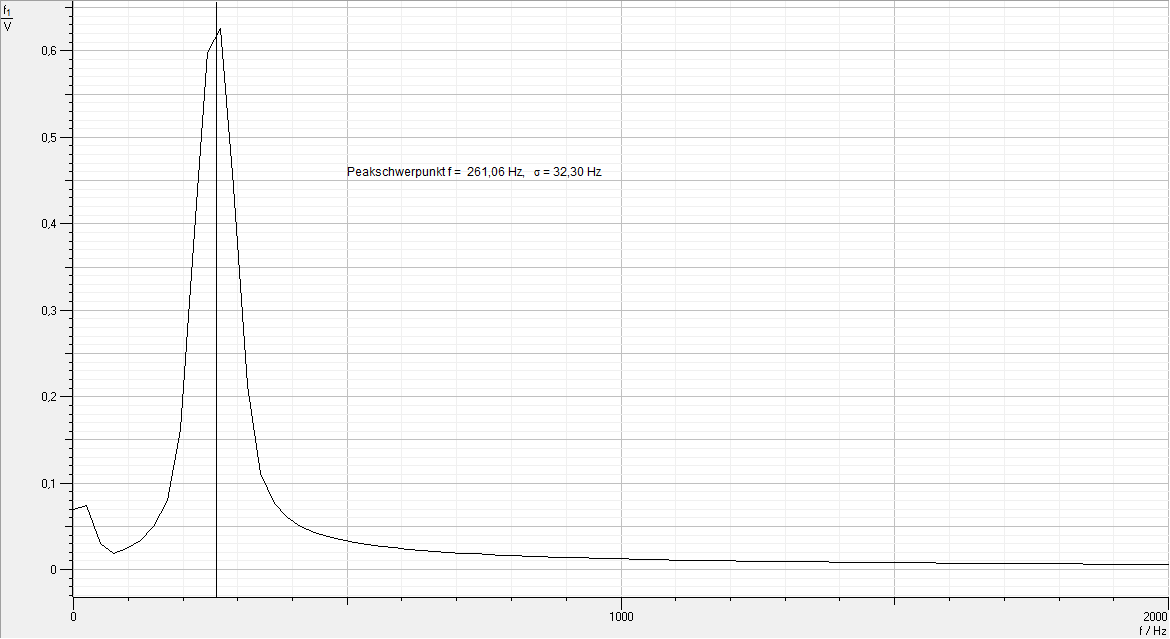
\includegraphics[scale=0.4]{Bilder/PEAK.png}
\end{figure}
\begin{equation}
f=261.06 Hz, \hspace{1cm} \sigma=32,3 Hz.
\end{equation}
Allerdings ist die Fehlerrechnung durch FFT fehlerhaft und undurchsichtig, die Fehlerabschätzung durch FFT ist also nicht sinnvoll. Im Folgenden haben wir die Frequenzen durch Ablesen bestimmt, um so auch den Fehler auf die Frequenz sinnvoll zu bestimmen.
\newline

\textbf{Bestimmung der Frequenz und des Dämpfungskoeffizienten durch Ablesen}: \newline
Wie bei Teilversuch 4.4.1 kann man die Frequenz und den Dämpfungskoeffizienten auch durch Ablesen der Maxima errechnen. Wichtig ist es auch hier den Offset vernünftig zu bestimmen und vor der Logarithmierung zu korrigieren.

\begin{figure}[H]
\caption{Messung der Minima und Maxima}
\centering
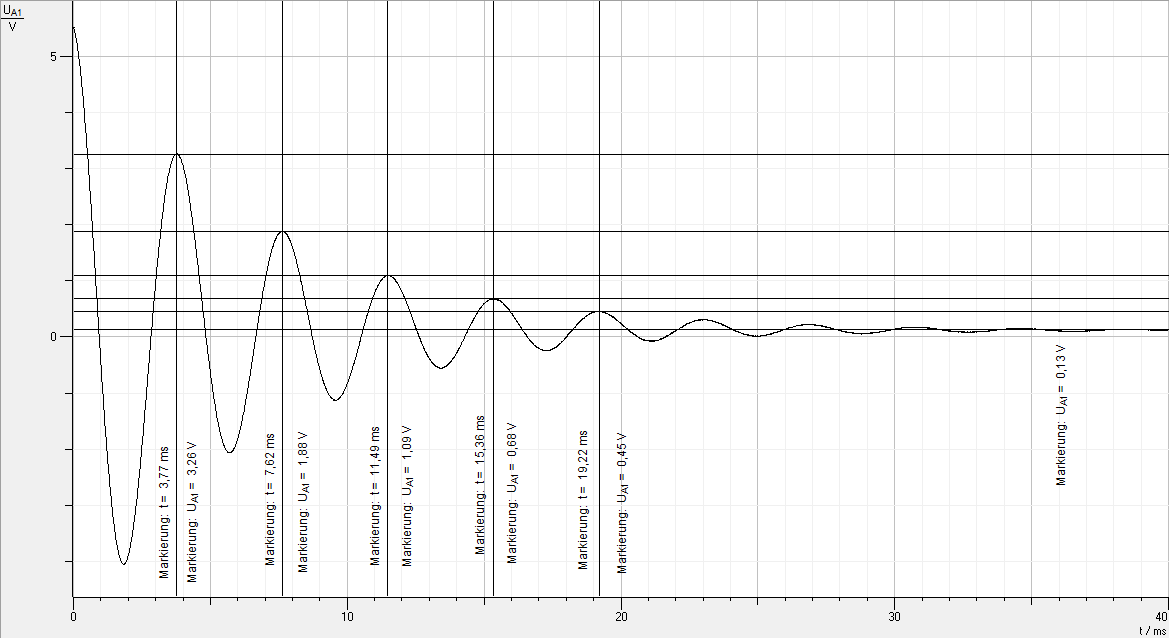
\includegraphics[scale=0.5]{Bilder/Einhuellende.png}
\end{figure}

Auf eben diese Weise haben wir 4 Schwingungen bei unterschiedlichen Widerständen vermessen.  Aus diesen Werten wurde jeweils die Frequenz und die Dämpfungskonstante mit Fehlern durch die Methode des gewichteten Mittelwerts bestimmt.\newline
Theoretisch können die Werte auch durch die Relationen:
\begin{align}
f_{Theo}&=\sqrt{\frac{1}{LC}-\frac{R^2}{4L^2}} \\
\delta_{Theo}&=\frac{R}{2L} 
\end{align}
bestimmt werden. \newline
Ergebnisse:
\begin{center}
\begin{tabular}{c|c|c|c|c|c|c}
R in $\Omega$ & $\bar{f}$ in Hz & $\sigma_{\bar{f}}$ in Hz & $f_{Theo}$ in Hz &  $\bar{\delta}$ in $\frac{1}{s}$ & $\sigma_{\bar{\delta}}$ in $\frac{1}{s}$  & $\delta_{Theo}$ in $\frac{1}{s}$ \\ 
\hline 
0.02 & 258.896 & 0.290 & 264.422 & 150.997 & 0.527 & 132.222 \\ 
\hline 
2.4 & 258.398 & 0.334 & 263.951 & 175.023 & 0.654  & 165.278\\ 
\hline 
5.5 & 257.046 & 0.331 & 263.178 & 225.027 & 1.050  & 208.333\\ 
\hline 
11.8 & 254.030 & 0.395 & 261.046 & 285.786 & 1.552  & 295.833 \\ 
\end{tabular} 
\end{center}

\textbf{Bestimmung der Induktivität}: \newline
Aus Relation (\ref{Spule}) folgt, dass die Steigung $a$ einer Geraden von $\delta$ gegen $R$, $a=\frac{1}{2L}$ entspricht.
Trägt man nun unsere Messwerte von $\delta$ unter Betrachtung der Fehler (Lineare Regression) gegen $R$ auf, ergibt sich der folgende Graph.
\begin{figure}[H]
\caption{Bestimmung der Induktivität mittels Linearer Regression}
\centering
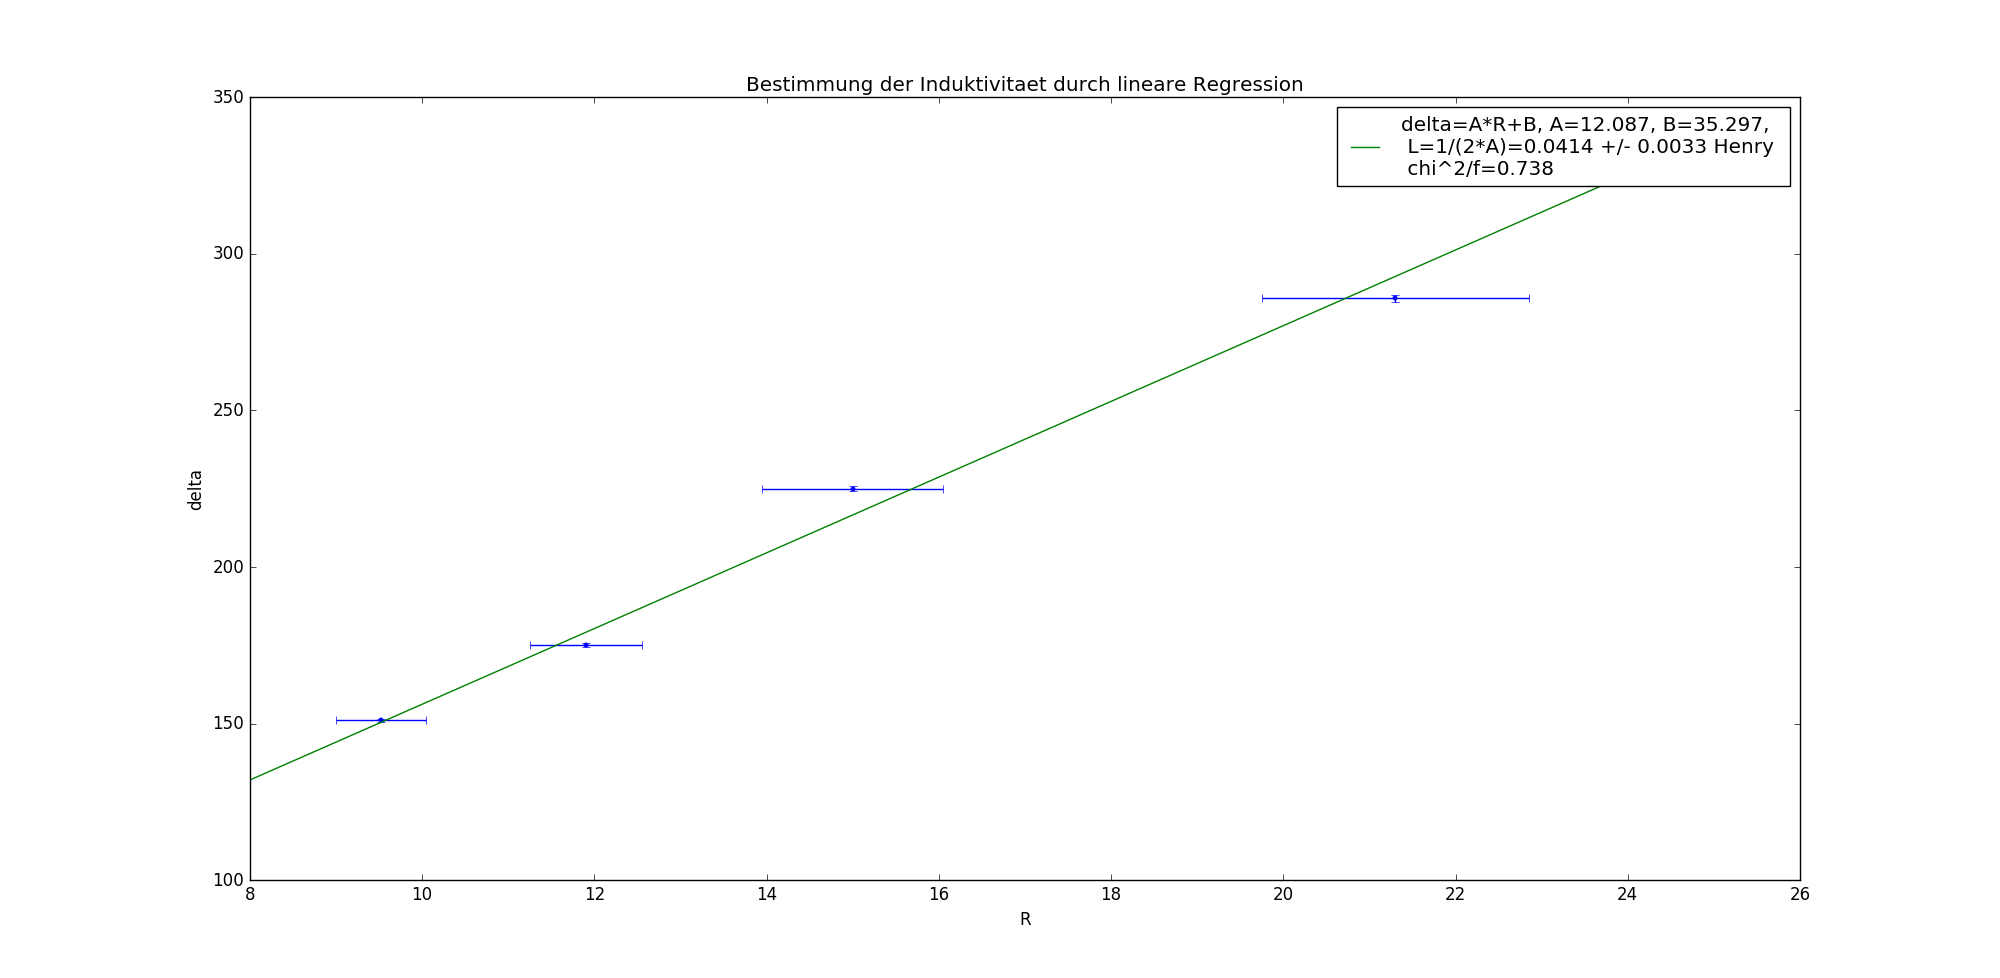
\includegraphics[scale=0.3]{Bilder/Induktivität_linreg.png}
\end{figure}
Der Fehler auf die Induktivität pflanzt sich dabei folgendermaßen fort:
\begin{equation}
\sigma_L=\frac{\sigma_A}{4A^2}
\end{equation}
Ergebnis:
\begin{align*}
\delta(R) &= A*R+B \\
A&=12.087 \frac{1}{H} \hspace{1cm} B=35.297 \frac{1}{s} \\
\Rightarrow L&=\frac{1}{2A}=0.0414 \pm 0.0033 H, \hspace{1cm} L_{Hersteller}=0.036 H\\
\frac{\chi^2}{f}&=0.738
\end{align*}




\subsubsection{Analyse und Fazit}
\textbf{Aperiodischer Grenzfall}
\begin{figure}[H]
\caption{Aperiodischer Grenzfall}
\centering
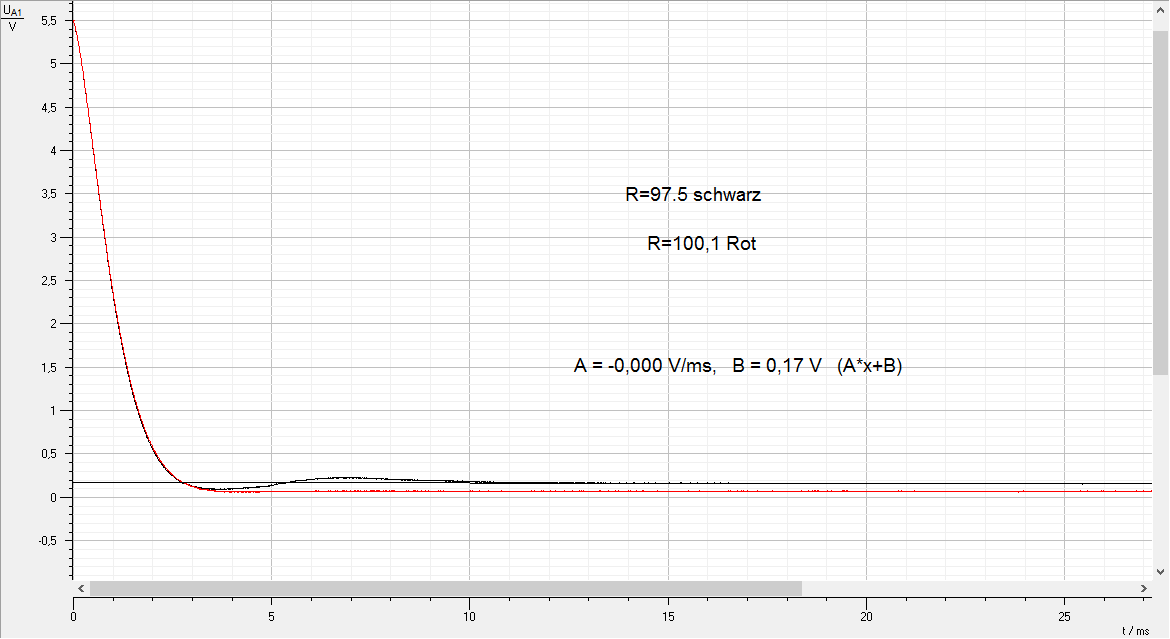
\includegraphics[scale=0.5]{Bilder/AperiodischerGrenzfall.png}
\label{Aperiodisch_Bild}
\end{figure}
Wie bereits erwähnt sollte der aperiodischer Grenzfall bei einem Widerstand von etwa
\begin{equation}
R_{ap}=2\cdot\sqrt{\frac{L}{C}}-R_{L}\approx 120\Omega - 9.5 \Omega=110.5\Omega
\end{equation}
aufteten. Mit $R_L$ dem Spuleninnenwiderstand.
Wie man in Abbildung \ref{Aperiodisch_Bild} sehr gut sieht schwingt die Schaltung bei $97.5\Omega$ noch, während sie bei $100.1\Omega$ gerade nicht mehr schwingt. Wir bestimmen den nötigen Widerstand für den aperiodischen Grenzfall also zu:
\begin{equation}
R_{ap}=100.1\Omega .
\end{equation}
Dieser Wert ist kleiner als der erwartete Wert, was aber zu erwarten war, da die Schaltung wahrscheinlich noch weitere Innenwiderstände hat als nur den auch sehr ungenauen Spuleninnenwiderstand.

\textbf{Analyse der Frequenz und des Dämpfungskoeffizienten durch Ablesen}: \newline
Betrachtet man die Frequenzen fällt auf, dass die berechneten kleiner sind als die theoretischen. Dies resultiert offenbar aus einem systematischen Fehler, denn die theoretischen Werte haben wir allein aus den Herstellerangaben für L, C und R berechnet. \newline
Der Fehler auf die Frequenz steigt mit steigendem R.
Dies kann man dadurch erklären, dass bei steigendem R die Dämpfung größer ist und somit weniger Maxima bzw. Messpunkte zur Verfügung standen.
\newline
Die Dämpfungskonstante steigt natürlich mit steigendem R, weil $\delta=\frac{R}{2L}\Rightarrow \delta \sim R$.
\newline
Diese Proportionalität pflanzt sich auch auf den Fehler von $\delta$ fort und erklärt somit auch das mit steigendem R steigende $\sigma_{\delta}$.


\textbf{Analyse der Induktivität}: \newline   
Bei der Linearen Regression kann man erkennen, dass  die Gerade alle Fehlerkästen schneidet. Der Fehler auf R ist dominant, was zu erwarten war, da wir ihn nur grob mit dem Drehwiderstand eingestellt und mit dem Multimeter überprüft haben (Fehlerabschätzung $\sigma_R=5\%$). 
\begin{figure}[H]
 \caption{Residuenplot für Induktivität}
 \centering
 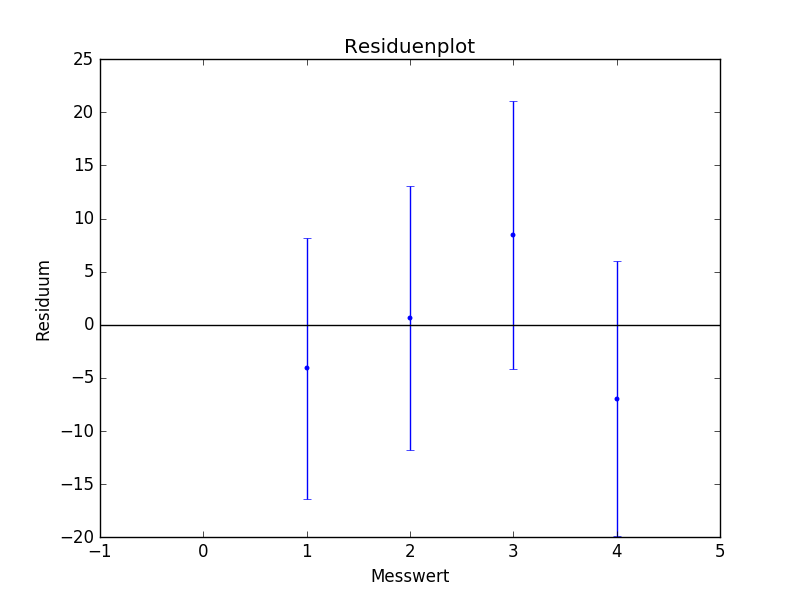
\includegraphics[scale=0.5]{Bilder/ResiduenplotInduktivitaeten.png}
\end{figure}
 
Der Residuenplot zeigt sowohl, dass keine Systematik vorliegt als auch, dass alle Werte mit ihren Fehlern passen. Auch das $\frac{\chi^2}{f}$ von $0.738$ ist passend. \newline

Der gemessene Wert für L ist kleiner als der theoretische. Dies lässt sich dadurch erklären, dass $L\sim R$ und wir wieder annehmen müssen, dass der Innenwiderstand  des gesamten Stromkreises als größer anzunehmen ist.

\textbf{Fazit}:\newline
Zusammenfassend kann man sagen, dass der Versuch äußerst erfolgreich verlaufen ist. Zwar weichen die gemessenen Werte oft von den theoretischen ab, die theoretischen Werte wurden allerdings auch nur aus den Herstellerangaben berechnet. Daher gehen wir davon aus, dass die von uns gemessenen Werte besser sind als die theoretischen.  
\end{document}